\setcounter{figure}{0}
\renewcommand{\thefigure}{9-\arabic{figure}}

\section[第九章\q 论坛文集]{第九章\\ 论坛文集}

这本书之所以能够最终出版，离不开众多网友的支持与鼓励。能够有幸认识这么多志同道合的朋友，得益于多年来通过论坛发帖与大家进行交流。最终，在大量热心网友的无私帮助下，我们创建了属于自己的交流平台——“交易者之家”。我很珍惜同大家一起经历过的一切，以及在交流中所得到的宝贵启发，同时更加感谢管理员“清醒的疯子”与广大热心会员的长期支持，大家的共同努力才使论坛发展到现在。

前面已经谈论了很多理论上的东西，而完全脱离实战似乎又会使本书多少有些欠缺。那么为什么不在本书的最后，附上一些曾经在论坛上发的帖子呢？或许，这样有助于大家更加清晰、动态地理解我的思维方式。这些文章很多都是发表在多年之前，或许文中的观点不免有些幼稚。但无论如何，这都是我走过的成长轨迹。

有一点我必须解释清楚。本书摘录的文章具有预测性质的部分，大家应该重点关注我的思维方式，而不是惊叹预测的准确性。装神弄鬼没有任何意义，这些只不过是我比较满意的一些文章。事实上，我仍旧发表过很多错误的市场观点，只不过大家在本书中没有机会见到罢了。比如，我很早就认为房价会下跌，但金融危机以后房价却大幅度地上涨。而更多的观点要么是无所谓对错，要么就是在时间上不存在任何实战价值。

或许，大家还可以换一个角度来思考预测的价值。我可以诚实地告诉大家：2005年998点的底部区域我的确预测出来了，但建仓仍旧是采用连续不间断趋势跟踪系统。我是通过付出两次止损成本后，才实现完美的战略性建仓。问题是，只要我甘心付出这两次成本，即使不进行任何预测，都是可以实现这种效果的。更有趣的是，即使我在底部形成之前，把牛市的升幅看得比几乎所有人都要大，但市场巨大的真实升幅仍旧大大超出了我的预料。事实上，我在1700点以后就开始转战期货市场，从而并没有在壮观的大牛市中赚到多少钱。接下来在2007年6124点的顶部区域时，我仍旧对大盘的顶部区域作出了准确的判断。而这种准确判断的价值，也不过是在大熊市中没有亏损一分钱罢了。要知道早已转战期货市场的我，是不可能在股市中赔钱的，而无论我是否能够预测出顶部。最后在2008年的底部区域时，我不但准确地的预测出底部，甚至拿着在金融危机中做空商品期货的利润，重新回到阔别多年的股票市场来抄底。更有意思的是，无论是买入的行为，还是对于指数升幅的预测，甚至是对市场热点的把握，都可以用近乎完美来形容。但最终我只不过赚了60％左右的利润，而大量的利润都被我放跑了！很遗憾，我在2009年2月的调整中仓皇而逃，从而做出了一笔荒唐透顶的“战略性离场”。

与此相对应的是，我在期货市场上赚到了更加庞大的利润，而这些利润大部分都来自于我无法预测的行情波动。很显然，市场是否能够被预测是一个问题，而预测是否具备相对于系统的价值又是另一个问题。2008年的底部区域时，我的确做了两件“不可思议”的事情：一件是在没有发出买入信号之前就通过信心十足的主观判断实现了战略性建仓；另一件就是鼓动身边的好朋友跟着我一起去勇抄股市大底。或许正是这种自负的主观判断，为我最终在调整中仓皇而逃埋下了伏笔。事实上，如果我坚持按照系统来应对股票市场，那么我能够获得的利润将要多上几倍！预测还是不预测，这个问题还是留给大家来思考吧。

\subsection{股市中还有一种叫做“牛市”的东西（2005.02.11）}

最近我发现各大论坛中的空头言论非常之多。止损跑出来的人开始沾沾自喜……我突然有一个想法，也许会对大家有所帮助。市场总会给首先相信“真理”的人一些甜头，但是随着“真理”的信徒越来越多，市场总会有收网的那一天。昨天我看到一篇非常好的文章。其中介绍了止损的重要性；下跌市道中“赚股票”也是一种策略；以及中金通过做空股市实现获利的模式。但是我始终觉得现在说出这些真理，也许对一部分人可能存在一些不良影响。我必须澄清一下：我对文章中的理念非常认同，没有否定、甚至攻击的意思。其实即使在大牛市中我也止损，这种方式很适合我。但对于已经数年进行“被动长期投资”的套牢一族来说，现在止损的目的，绝对不会是下跌两百个点就马上回补的，更不可能甘心以更高价位买入！9·14行情失败以后，我在1290点实现战略性空仓。但我并没有建议我身边的人也空仓。因为如果我看错了，我有控制损失的能力。可大多数人却未必有这种认错的勇气。以下是我对这篇文章的回贴，希望能够对大家有所帮助。

好文章阐述的道理既简单，又非常重要。可惜很多股民在大盘高位时，就是不明白“赚股票”这样简单的道理！但有一点我必须指出：本文的观点确实是对过去数年股市走势的深刻总结，也是实实在在的真理。请注意“过去”这两个字。任何真理都有它的发扬光大和付出成本的时期。止损或者“赚股票”的道理现在没有哪个股民不明白（但愿数年以后大家不要忘了这个简单的道理）。看看各个论坛中盛气凌人的空头言论大家就会明白。现在的问题不是止损的纪律是否有用，而是大众有没有止损的勇气？或许相当一部分人已经拿着亏损的筹码暂时离开了股市（不获利绝对不抛出）。也许另一部分人已经止损（而开始感到庆幸），或者操作开始非常谨慎了。

我们回顾一下历史上各个时期的主流投资理念吧：1997年初，注重业绩长期持股是股市获利的关键！买入长虹、发展（绩优股）只赔时间不会赔钱。5·19行情前期，某著名分析师指出：中国股市已经步入熊市。并且告诉我们的道理就是止损的重要性，以及大部分人在牛市时很难赚回熊市时亏损的钱。2001年初，在面对缓慢上涨的大盘时，对于众多股民反复操作、却常常亏损的现状，专家提出：长期投资是股市获利的关键，并指出应该树立长期投资的投资理念。

请问在2000年以后，中国股市数次快速下跌，而又有惊无险地被拉起时，你有没有勇气大谈止损的真理？即使你这样做了，结果也是一次又一次遭到市场的嘲笑！当最后你没有勇气说出真理的时候，中国股市真的崩盘了（其实我就是这样）。经验是对过去行情的总结，但用这种由过去行情总结出来的经验应对未来的操作时，就显得非常可笑了。

其实楼主的观点我非常认同，对于“赚股票”的道理也非常理解（其实以前我很热衷于赚股票；而现在我空仓并不是为了赚股票，而是为了过滤出强势股）。我从1783点至今至少空仓8个月，只亏损了（9·14行情时）千分之几。到目前为止我还是空仓（如果未来股市继续走好，我会马上战略性建仓）。但我现在已经不再说止损的观点了，太晚了！也许坚定信心的言论对投资者更有用！

2005年上半年肯定能形成结束2245点以来大熊市的终点，一浪上扬肯定会走出（别误会，不是主升浪）。以前我认为调整的极限是1025点，现在我正在准备用事实（未来几天股市的走势）验证，1189点是不是最终底部。总之，现在还是多想想股市中还有牛市吧。多想想2001年时，大众用巨大代价总结出来的真理吧。这些只是个人观点，希望不要影响大家的思路呀。

\subsection{狼来了，狼来了（2005.03.21）}

每个人小时候都应该听过《狼来了》的故事。在股市上，这个小时候的故事却被一次一次地上演。其实，小时候的很多寓言故事说明的道理，都很适合分析股市中的问题。比如《农夫和金鱼》里面，那个贪得无厌的农夫太太，从贫穷到富有，再到极其富有，最后的结局却又变回了一无所有！当一轮长期牛市过后，我们和那个贪婪的农夫太太好像没有任何区别。好了，不说题外话了，我们还是来主要说一下股市中《狼来了》的故事吧。

1999年的5·19行情涨势如虹，几乎走成了一条直线，但其中也有两次恐慌的单日下跌，收出了实体很长的长阴线。第二天开盘后，股指就重回升势，结束了单日洗盘行情。这种洗盘真的是很成功，至少对于主力有两个明显好处：第一，可以将持仓不坚定的筹码震出，从而提高散户的平均持股成本；第二，可以告诉大家一个简单的道理，快速的大幅下跌并不可怕，甚至是逢低吸纳的大好时机！正是由于主力教会了大家下跌并不可怕，所以在7月1日那根宣布5·19行情结束的大阴线面前，很多股民已经不再害怕了。

2000年的大牛市，在达到2245点以前有三次大幅跳水后又被拉起的走势，每一次跳水都非常恐怖，都将中期重要支撑均线跌破！虽然时间跨度比5·19行情长了很多，但是其中的奥秘和道理却是完全一样的。遗憾的是，《狼来了》这个故事中被狼吃掉的是“说谎的放羊娃”，可股市上被狼吃掉的却是善良的人们！也许一个大牛市，就是给刚刚学会止损的投资者上课！告诉他们，止损是非常可笑的！善良的人们一次一次被狼来了所欺骗，最后狼真的来了的时候，却已经没有一个人肯相信了。

回到现在的股市，其实也是在上演一部“狼来了”的闹剧。当然我没办法肯定哪次狼会真的到来，但我知道狼总有一天真的会来！9·14行情以失败告终，这似乎是第一次告诉大家：在大熊市中不要有过多的奢望，逢高减磅是永恒的真理。没有在高点卖出的投资者，肯定会后悔不已。1187点开始的反弹行情，似乎又要以失败告终。这再一次告诉大家，不要对大行情抱有任何幻想。

也许大家真的会像善良的人们一样，两次中期牛市的希望破灭后，已经不会再相信股市中还会有什么中期牛市行情。下一次等股指再短期快速上扬后，一定要吸取前两次的教训而卖出股票！但我的思维方式正好相反：如果说9·14行情演化成中期牛市的概率是“1”，那么1187点的行情演化成中期牛市的概率就是“2”；下一次反弹行情演化成中期牛市的概率就是“4”；如果下次又是以失败告终，那么再一次的反弹成为中期牛市行情的概率就是“8”！希望大家能够明白我说的道理，通过《狼来了》的故事得到一点启发。

\subsection{现在什么最可怕（2005.05.10）}

今日盘中最低点为1108点，正好封补了5·19行情中的第一个跳空缺口。同时中集集团在今日的盘面中，也确实出现止跌。中集的跳水至少在今天并没有扩散到整个基金重仓蓝筹股。似乎这一切都是相对偏好的迹象。

这两天的盘面确实非常恐慌。很多朋友也打电话问我今后的行情会怎么走。说实话我也不知道，所以没有给出正面的回答。其实就在这两个交易日，我已经差不多送回了这两个多月以来形成的利润。大盘真的会崩盘吗？冷静地想一想，虽然我还有很多向好的理由，但真的不会出现意外吗？

单单从指数上来看，如果再创出1108点的新低，那么我已经在技术分析上找不到任何看多的理由。同时很多支撑线都处于略微跌破的状态，当然现在还是可以一厢情愿地认为只是短时间的假破位。从个股阶段分布来看，现在确实显示出一轮长期牛市即将产生。难道这次的预测错了吗？现在认错还有些过早。但是大盘的短期趋势如果不扭转，那么距离我承认错误已经没有几天的时间了。

现在的我，信心与迷茫同在。接下来应该怎么办呢？记得我说过：在系统允许的范围内，我可以展开自己的想象力，相信自己的预测。但现实超出系统能够容忍的范围时，我会放弃预测而相信自己的眼睛！对我来说，接下来的操作反而在迷茫中变得简单。我从现在开始转换为机械的操作方式。今天我已经对三只持股制定好明确而机械的止损点。今天收盘时看了一下资金，还有3600元的利润。粗略计算了一下，触及止损点时的亏损应该不会超过5000元。哈哈，现在我只能听天由命了。

难道这次战略性建仓真的和9·14行情一样，又以失败告终吗？机械的止损会不会在大盘的最低点被触及？其实这些都不重要！大不了再以更高的价位买回。只要大盘不继续振荡，那么无论向上还是向下，无论我的止损对错与否，我都会是赢家！

言归正传，现在股市中最可怕的是什么？对我来说，什么都不可怕。但是最近两天我调查了一下股民们的心态，他们的心态才是最可怕的。昨天大家期待反弹放货，今天大家却说“反正这么低了，爱怎么样就怎么样吧”。真是太可悲了，涨跌皆输的思维呀！

对于我自己的理念而言，我仍然坚决看多。但也许在几天之后，我会卖出所有的股票。如果现在大盘是底部，那么做空可怕吗？我要说做空不可怕！如果你有牛市思维，即使1999年你在1047点做空也不可怕！大不了被扎空一百多个点，没什么了不起的。最可怕的是：无论你现在满仓还是空仓，只要你被这4年大熊市折磨得已经全是根深蒂固的熊市思维，那么无论怎样都是最可怕的。

这4年大熊市中形成的熊市思维和最近8个月形成“反弹后继续创新低”的定势思维，已经注定了散户投资者在股指运行到1200点到1300点之间时，会涌现大量“散户抛盘”。主力的选择只能是高举高打走出大牛市；或者马上崩盘，从而套牢期待反弹放货的中小投资者。

我坚信，有强大的理由坚信：无论如何5月份都会选择突破方向，无论是崩盘还是主升浪；无论如何2005年都形成4年大熊市的最低点，这一点无论是5月份的1100点左右还是7月份的800点左右。预测行情并不重要，预测的正确与否也不重要，重要的是你必须明白你的操作是在赌什么。

\subsection{生物进化与炒股方法（2006.04.08）}

我是一位股民，但同时小时候也是自然科学的爱好者。聊现在的行情，我可能和很多人没有什么共同语言。无聊当中不如聊聊自然科学和股市共同适用的哲学思想。我更希望找到事物的本质，看看生物进化与炒股方法之间是否有相似之处？建议大家把生物部分与股市部分对照着看，这样才能看完这篇无聊的文章。

生物的生存方式与股民的交易方式是否存在一些相似的东西呢？这确实是一个奇特的想法，但他们确实存在某些相似性。生物的生存方式是为了适应自然的特征，而炒股方法是为了适应市场的特征；自然特征是变化的，而市场特征也是变化的；生物使用不同的生存方式来应对自然，而股民也是用不同的炒股方式来应对市场；生物为了争夺自然资源，而股民也是为了争夺市场资源；生物之间是共存的，而股民之间也同样是共存的（否则就无法成交）。

关于生物进化的正统理论是达尔文进化论。达尔文讲述的是以物种通过偶然突变为依据的自然淘汰说，这方面大家都知道我就不多说了。但近年来对达尔文进化论的质疑越来越多，似乎越来越多的进化现象是达尔文进化论所解释不了的。好在我无意探讨进化理论，而只是想从生物进化的特征入手，谈谈其与炒股方法的相似之处。

\textbf{第一，部分生物进化存在“癖好”倾向。}熊猫只爱吃竹子，树袋熊只吃桉树。事实上这是适应性极差的物种，只要竹子和桉树从地球上消失，大熊猫和树袋熊就会灭绝。相对来讲，老鼠几乎什么都吃，它们的适应性是极强的。那么，自然淘汰说为何既让强者活下来，又让弱者活下来呢？事实上，自然界的所有生物并不是选择效率最高的方式来应对自然，它们存在着某种特殊的“癖好”。上帝为什么创造出这种对环境要求极高的生存方式脆弱的物种呢？

\textbf{第二，部分生物进化存在“复杂”倾向。}生物为了达到一个简单的目的，而选择了极其复杂的方式。这是一种表现欲吗？事实上，这种复杂并没有高的效率。比如有一种名叫肝片吸虫的寄生虫，它的循环周期非常奇特：当肝片吸虫尚未成熟而被绵羊粪排出体外后，它必须在一种小鱼身上生长一段时间，然后再在一种小贝壳内生活一段时间，最后又重回到绵羊身上。在小鱼和小贝壳身上，它都会成长一个阶段。因此，它的成长过程是很艰难的。一个肝片吸虫会产生1500万个卵，而100万个卵中只有一个能够顺利长大。要知道其他寄生虫的生长周期都是相当简单的。也就是说，自然界最复杂的机制是同最简单的机制并存于世的。再比如，花朵的授粉也有不同的机制，有的非常简单，而有的又极其复杂。其中一种兰花并不分泌花蜜，而是靠形状酷似昆虫来引诱胡蜂。更有意思的是：有些地区，生长着一些古怪的蜂。雌蜂不许雄蜂靠近，因为雄蜂身上没有可以吸引自己的特殊气味。但偏巧在这些地区，生长着一些这样的兰花。它们能分泌出一种粘液，这正是雌蜂所需要的气味。这样雄峰便纷纷落在这些兰花上，从而有了雌蜂所需有的气味，同时帮助兰花授粉。

以上是一位法国生物学家在《意志的生物学》中所举的例子，目的是质疑达尔文的进化论。我无意探讨什么进化论，只是说一些生物生存特征的一些规律。事实上，部分生物为了达到非常简单的目的，而采用了非常复杂的方式。没有人知道造物主为什么会有这样的偏好，但这确实是真实存在的。此书还列举了很多这样奇怪的案例，来阐述这样一个道理。生物的进化有趋向复杂的倾向，他将其称为“表现欲”。这说明进化并不是没有方向的，而是趋向复杂。他将鱼类身上存在着一种想变成青蛙的东西称为“意志”。也许正是这种复杂化的意志，才让生物从单细胞生物进化到人类这样复杂的生物。但一个问题必须注意：这种复杂的探索失败率是非常高的。比如，马的祖先原马是在白垩纪末期诞生的，这个始祖又分成许多分支，在每一分支上都发现某些马的特征。在一个分支上，它的蹄子像马，而头根本不像马；在另一个分支上，它的蹄子不像马蹄，但头却像马头。这是物种进化的摸索，但最终存活下来的却只有现在的马。马一直在显露自己，但最后只有一个分支成功了。

\textbf{第三，部分生物有过度适应环境的倾向。}想想也好笑，在我们这个地球上存活时间最长的物种，恰恰是从来都没有风光过的物种。与此相反的事例就是恐龙，它们很快灭绝了。这样我们可以想象出一种假设。某物种极度适应当时的自然环境，并且快速发展壮大自己，最终争夺到自然界更多的生存资源。但问题是：一个物种如果越适应当时的自然环境，那么它很可能就越不适应变化后的自然环境。相反，能够长时间适应自然环境的物种，似乎并不可能极度地适应某一特定时间的自然环境。

\textbf{第四，自然环境和物种进化存在某种循环吗？}考古学家已经证实，在过去的数亿年里，地球经历了几次冰河时期，那么相对应的也就会有几个温暖潮湿的时期。同时物种经历过几次集体灭绝，还有几次物种大爆发。这其中确实存在某种循环，但这种循环是否存在某种规律呢？我们不谈循环的成因，只谈论一下循环的规律。这种循环并不像春夏秋冬四季循环那样，具有某种特定的时间周期。从时间间隔上来看，并不存在绝对的时间周期，但又似乎具有某种非常模糊的周期。这一点很像股市的繁荣与萧条，它们确实是在循环，但并不存在绝对的时间周期。同时我们肯定股市的萧条后会迎来繁荣的阶段，但我们又不能预测出具体的时间和幅度。

说到物种灭绝，我们就不能不谈一下恐龙那次集体灭绝。按照大众接受的说法，小行星撞击地球使恐龙出现了集体灭绝。但《临界》这本书又提出一种新的观点。该书指出物种灭绝每天都在产生，物种灭绝的规模呈现出能量分布法则的特征。这就好像地震每一天都要发生几次，但大地震并不常见。它们形成的原因是相同的，只不过越大的地震发生次数就越少。不同强度的地震之间，在数量上存在某种严格的比例关系。而物种灭绝被我们观察到的是集体灭绝和背景灭绝（每天都在发生而不被我们重视的灭绝），这就好像是大地震和背景地震。每一种物种的灭绝都可能影响到其他物种，如果地球上没有了竹子，熊猫也就会没有了。也许自然界的生物链不存在绝对不相关的物种，那么物种灭绝就像是雪崩。只不过有的雪崩很快停止了，而有的却演化成灾难。

我不想探讨这两种解释谁对谁错，这不是我能力范围以内的事情。我个人感觉，他们从不同的角度阐述了物种灭绝的现象。也许他们都对，而上帝却让他们配合得恰到好处。小行星撞击地球应该是对物种灭绝直接原因的解释，而能量分布法则是对物种灭绝规律的表述。就好像本次大熊市也许有其特定的原因，但同样符合能量分布法则。换言之，没有这样的理由，也会有那样的理由。人类能够给任何发生的事情找到理由，即使这种理由不一定正确。也许特定的事情并不一定需要特定的理由。西方谚语中“压倒骆驼的最后一根稻草”，并不需要是最重的。我们的世界存在着“封冻”原因的机制，这可以使原因并不直接产生作用，而到一定程度才会释放出来。

\textbf{第五，为什么上帝没有创造无敌病毒？}2003年的“非典”病毒席卷全球，这时每一个人都对病毒增加了关注程度。病毒只是一个基因密码，这么简单的东西居然是几乎唯一（还有细菌吧）能够对人类构成威胁的生物。它虽然很可怕，但站在病毒的角度上来讲它们没有一个品种是完美的。比如，天花的克星是牛痘；艾滋病虽然是致命的，同时潜伏期很长，但他的传播能力很弱；“非典”病毒的杀伤力很强，并且传播能力很厉害，但它的潜伏期很短，这样就可以很好地控制；还有一种曾经在东南亚爆发的病毒（忘了名称了），也很致命，但它有一个“缺点”，就是只能从动物身上传播给人，而人与人之间是不传播的。

如果上帝创造出一种病毒，它具有艾滋病的潜伏期和杀伤力，同时具有“非典”病毒那样的传播能力。那么人类会怎么样？很难想象吧？为什么上帝没有创造无敌病毒，我不知道。但我知道，造物主没有让任何一个物种达到完美的程度。任何事物都有弊端和弱点，也许这才是整个游戏进行下去的前提。如果对手不存在了，你也就不存在了。也许这就是上面问题的答案。事实上生物的进化不光是竞争，还有合作的产生。这方面我依然能够举例说明，但还是不浪费篇幅了。

上面探讨的是生物进化和生物生存方式的几种规律。这些规律说明什么问题并不重要，这些事情还是留给科学家去思考吧。下面我们看看股民们的炒股方法是否也存在着与此对应的规律呢？

\textbf{第一，部分股民在炒股方法上存在“癖好”倾向。}说到这，我不能不谈一下在《短线交易大师：工具和策略》中讲到的一个故事。作者某日接到一个电话，一位客户说他留意了很长时间贵公司推荐的股票，事实上他们经常是正确的。但是这对他没有意义，根本没有一点的好处。为什么呢？因为他们推荐的股票通常都是正在上涨的股票，而那位客户想要的是正在下跌的股票。同样在我身边的股民中，有的人不会去买入市盈率高于30倍的股票，这使得大量的利润无人认领；还有的人不会买入10元以上的股票，而只喜欢价位低廉的股票。

事实上，很多股民正在因这种“理所应当”的癖好流失自己的金钱。这种癖好到底能够产生什么样的结果呢？统计表明，正在上涨的股票未来继续上涨的概率要大于正在下跌的股票；同时股票能否上涨和市盈率的数值并没有必然的联系，但市盈率反复提高的股票未来上涨的概率要大于市盈率反复下降的股票；高价股和低价股在不同的市场阶段会表现出不同的强弱特征，也许这一段时间低价股走势好，而那一段时间高价股走势好。问题是概率上并不存在低价股上涨概率大于高价股的统计特征。事实上，至少很多黑马的中后期都是高价股，同时低价股下跌空间并不比高价股小。

为什么会这样？也许还是人类的本能吧。但事实上很多股民的癖好并没有统计学上的优势。任何方法都有成功的时候，我说的是统计学上的优势。以前对于正在下跌的股票我会说我看空，现在我会说我看不懂。事实上，它们也有马上大幅上扬的可能性。我希望更多的股民所使用的设置是建立在统计学基础上，而不是建立在癖好上，或者只是一次成功的操作经历上。不过如果大熊猫不是只爱吃竹子而是什么都爱吃，那么很可能它就不那么可爱了。哈哈，那是令人讨厌的老鼠。不过我们要的是利润而不是可爱。

\textbf{第二，大部分股民有采用复杂炒股方法的倾向。}我所说的这种复杂同生物的生存方式一样。为了达到一个非常简单的目的，而使用一种非常复杂的方法。如果想想生物复杂化的本能，也就能够理解人类为什么要追求复杂了。这种复杂是推动生物进化的动力，但你是否想过这个问题？如果你现在采用单细胞式的简单方法就能适应市场环境而实现获利的话，那么你还有必要，通过“试错”把你的炒股方法在你的有生之年，从单细胞生物进化到人类吗？并不是每一个物种都能成功地进化到人这样复杂的生物，而其中为了复杂而淘汰的物种也许真的不计其数。像上面的那种肝片吸虫，只要一个环节出现问题，它就会退出历史的舞台。

不把话题扯远，我们继续说炒股。人类真的有把简单事情变复杂的天赋。很多人炒股就是在不断追求高难度动作。有的时候我在想，股民来到股市上是为了获利，还是为了追求成就感？股民们采用了越来越多的分析方法，但具有讽刺意义的是，他们却不会真的尊重其中任何一种方法。我个人觉得，一位股民成熟的第一部分是在不断学习方法，而同时又在不断忽视方法；而股民成熟的第二部分是不断忽略方法，而同时又在不断学会尊重方法。事实上，我现在炒股考虑的问题比5年前要少得多。我解释一下什么叫尊重方法。只有你尊重一种方法的时候，这种方法才会同样尊重你。我见过很多股民说：“我看空大盘，因为大盘已经跌破x日均线。”好，我问一个问题。你是否对于大盘每一次跌破x日均线时，都会进行空仓操作？没有！不可能这样！你总是对待一种方法呼来喝去，那么我可以想象这种方法会如何对待你。有意思的是，当你用x日均线作为机械的买卖信号时，并且通过真实的历史走势来检验这种方法的效果时，你惊讶地发现：原来这个简单的方法是一种可以获利的方法，至少比你过去几年的实际战绩要好很多。也许对待炒股方法也要做到，宽容地接受弊端。什么叫选择，选择就是权衡利弊。如果一种方法只有利而没有弊，那么你还用选择吗？

如果你学会尊重方法，那么你的策略就不可能复杂。为什么呢？如果你的方法，或者说策略中的设置超过5个，并且你又能够绝对遵守这些规则的话，那么你根本就会寸步难行。矛盾总会不断发生，对吧？以前关于复杂和简单的话题我谈论过很多，这里我不想再过多浪费时间。能够跟踪趋势已经是高手了，我们为什么要进行高难度动作呢？难道卖在天花板或者买在地板上的操作，真的那么具有诱惑力吗？我相信一位股民如果越成熟，那么谈论股票时的话题就会越少。而我见过很多股民滔滔不绝地说着股票，从国际形势，到国内大环境，再到公司的基本面，还有趋势分析、阻力位、支撑位等。我感觉真的是一脑袋糨子，思维根本就是混乱不清的。事实上，除非你进行原因的筛选，否则不可能挑选的原因都指向同一个结果！新股民还有一种倾向，你听，某某股票，*****7.6元、******7.42元，******6.38元……听得我头疼，根本就是“棒槌”嘛。记住，我们来股市不是为了做秀、不是为了戴上光环、不是为了让人羡慕、不是为了追求成就感、不是为了表现自己、不是为了坚持自己的癖好……我们的目的只有一个，那就是获利！

\textbf{第三，大部分股民有过度适应市场的倾向。}大盘从1783点跌到1067点（因为998点以后我依然亏钱），这段时间我的战绩如何？亏损20％多一点，我承认很多股民做得比我好。我见过这段时间1分钱也没有亏损的股民，也许还会有获利的股民吧。那么大盘从1067点到1340点这段时间我的战绩又如何呢？盈利50％，我相信依然会有很多股民做得比我好！但问题是，把这两段时间累加起来的战绩，比我好的人就不会很多了。如果放在更大的尺度上来观察，比我战绩好的股民可能会更少。这说明什么？这说明我并不想过度适应市场。我的方法并不是最适应熊市的方法，同样也不是最适应牛市的方法，也许我的方法是能活得更长的方法。

事实上，我并不追求过度适应市场，也就是并不希望让自己太风光。上帝想让谁灭亡，首先会让谁疯狂。如果假设我一段时间的利润是n万元。那么有几种组合实现这种利润的可能：10次盈利实现的；1次盈利实现的；1次盈利+3次亏损实现的。我会选择最后一种情况！也就是说，如果利润一定，我会选择更多亏损次数和更少盈利次数的那种方法。亏损本身就是一种对策略风险的释放。

什么是最适应熊市的方法？比如，一直空仓，对任何一次上涨都按照未来还会创新低的反弹来处理。事实上，从1783点开始的下跌中，没有亏损一分钱的股民就是这样做的。幸运的是，他成功地“扛”过了9·14行情和其后的每一次“反弹”。不幸的是，他也奢望“扛”过这次我认为是中期牛市的行情。前两个月他自信玩认沽权证，现在已经有一段时间在大户室没有看到他了。也许猜测底部买入，并且在上涨一小段以后卖出的方法更适应复杂的熊市，这样也许在过去的熊市中还能盈利！但市场特征一转变，你就会发现这种方法是多么的脆弱！从戴上光环到一落千丈往往就在一瞬间！也许成功的次数越多就越能加深操作者对这种方法的信心。但遗憾的是，这就距离市场变化的时间越近了！

大家是否发现这样一种现象？流传在这个市场上的投资方法和投资理念都具有这样的规律：一部分是数十年甚至上百年前产生的那种并不精确（概念上的）的东西，一部分是最近几年产生的那种复杂与精确的东西。并且在此之间的很多东西都慢慢被市场忘记了！记得有人在1997年以前发明了一种“小波浪理论”，当时抄底逃顶屡试不爽。但1997年以后的市场环境改变了，这种理论也就没有任何价值了。有意思的是，生活在我们这个地球上的物种中，有最近几千万年才脱颖而出的哺乳动物和比恐龙还古老的昆虫，但恐龙已经消失了！是否等到遥远的未来，地球上已经没有人类，但昆虫还是现在的昆虫呢？

\textbf{第四，我们的股市存在某种循环吗？这种循环的机制又是什么？}上面已经将股市的循环和自然界的循环作出了对比，这里我们就不再重复了。这里我想谈论一下这个问题：股市上的大事件一定需要特定的原因吗？我是说，我不想用小行星撞击地球说的思维方式来思考股市，而使用《临界》书中的思维方式来思考股市。我们可以说本次大熊市是由于股权分置的原因产生的，那么我有两个问题：第一，如果下次没有股权分置，是否就不会产生大熊市了呢？答案肯定是否定的！那么我们研究这种原因就没有意义了。也许恐龙的灭绝真的是由于小行星撞击地球，但下次如果小行星不撞击地球就不会出现生物集体灭绝了吗？这个道理是一样的，我们不谈论原因而只考虑规律。第二，如果股权分置发生的市场环境发生变化，那么产生的结果是否也会发生变化？记得1997年以前转配股出现的时候，大家都认为转配股上市的时候股市会走熊。但事实上，2000年转配股上市的时候，市场是走牛的，甚至转配股涨得更多！如果2001年以前大盘没有从1043点涨到2245点，那么股权分置是否还会形成大熊市呢？与其说是股权分置形成了大熊市，还不如说股市本来就该走熊了。只不过它起到了催化剂的作用，如果没有它熊市也会产生。泡沫的破灭是必然的，而使泡沫破灭的原因是偶然的。或许恐龙灭绝也是这样。

那好，我们继续探讨股市循环的特征。事实上，股市的波动也是符合能量分布法则的。越大的波动发生的次数也就越少。大事件或者说大波动并不需要大的原因。其实趋势跟踪系统就是靠偶然事件来盈利的，但更多的股民是因偶然事件而毁灭的。问题是这种偶然事件是必然发生的。

我们试着探讨一下股市循环的机制。股市的波动是随机的吗？这是上百年来市场分析家争论最多的话题，遗憾的是直到今天还没有答案。反对未来是可知者指出，到目前为止还没有预测行情的公式产生，市场总能够让最富有逻辑的预测感到尴尬。反对漫步随机者指出，漫步随机无法解释趋势的问题。如果我们用抛硬币的方式来绘制走试图（正面上涨一个格，反面下跌一个格），那么并不能产生股市上存在的持续的趋势。问题是，股市的波动以及一切自然现象似乎都具有这种特点，他们介于可知与随机之间。

我想起以前喝酒时玩过的一个游戏。就是一群人在饭桌上放6个酒杯和一个骰子，而这群人轮流掷骰子。由于每一个杯子都有一个对应的数字，掷骰子得到的数字都会对应一个杯子。如果杯子是空的，那么就倒满酒，轮到下一个人继续掷骰子。当然如果杯子是满的，那么就把酒喝下去，继续掷骰子，直到掷到空杯子为止。这样就形成了一种动态的平衡，而随机控制下的“趋势”产生了！因为总是有人会喝下很多杯酒。游戏规则会使结果形成某种模糊的规律，而整个游戏又是在随机的控制下进行的。也许我们的真实世界就是这样：在规律的设置下，由随机推动。这个游戏其实和《临界》中森林大火的模拟游戏是一样的。那是在电脑上模拟的一个游戏：在一个范围内每隔一段时间随机长出一棵模拟的树木，然后每隔一段时间随机出现一个火柴（模拟闪电）。如果火柴正好落在树木上就会引起森林大火，并且波及与此相连的树木。在树木稀松的时候，火柴只会引起小规模的火灾，这样树木就会往繁茂发展；在树木繁茂的时候，火柴就会引起大规模的火灾，这样树木就会往稀疏发展。这就是一种动态的平衡，而我们能够知道的就是：（1）森林火灾（小事件）时刻都在发生；（2）森林大火（大事件）早晚都会发生，同时并不需要特殊的理由；（3）我们并不能预测森林大火发生的规模和时间；（4）火灾规模符合能量分布法则：越大的火灾发生次数越少；（5）模拟的火灾和真实的火灾规律很相似。随机、循环、规律、大事件等都在这个游戏中体现出来。也许我们观察到的世界和我们的股市，本质上都是这个样子。甚至我们可以通过在游戏中设计更加复杂的规则，来模拟真实的股票市场。

顺便说一句，上面的解释只是来自于观察而不是能够揭示原理的理论。难道上帝真的是在掷骰子吗？这是相对论与量子理论的争论，同样谁也不能说服谁。好在我们是股民而不是科学家，这些事情同样留给科学家吧。未来是否是一定的？我不知道。但未来是无法计算的，我们都必须承认。也许有两种解释：（1）原因无法对应结果，那么未来就不是一定的。（2）原因对应结果，但我们不可能考虑到所有的原因。比如，我们不可能计算每一只蝴蝶扇翅膀对风暴的影响。也许未来对于上帝来说是一定的，但对于观察者来说未来一定是不确定的！分析（观察）时，我们只能相信原因与结果之间具有不确定性。

\textbf{第五，市场上存在完美的策略吗？}上帝都没有让任何一样东西完美的意思，那么我们又何苦去追求完美呢？我以前的文章一直讲述操作策略中缺陷产生的必然性，这里就不再多说了。其实任何一种方法在达到一种效果的时候，必然会失去一些什么。从单一的操作方法上来看，方法并不存在优劣之分，关键是看你如何把各个方法组合成具有一致性的策略。我一直以为止损是一个绝对的好方法，我是说对任何操作者管用。但事实上并不是这样。林奇好像就不是靠止损点来控制风险的，因为他是靠基本分析来取胜的。基本分析从本质上就与止损思想矛盾，那么他是如何控制风险的呢？很简单，分散投资。

这里我讲述一个故事，它来自于《幽灵的礼物》。该书作者是一个成功的日内交易者。在他前面有一位女士，她是做头寸交易的。作者总是把日内快速拉升的股票套现，而这时通常他的抛盘会被前面的那位女士接走。同时那位女士总是每次都说：“我不希望买入你的抛盘，因为这样我通常总是输。”有意思的是，一次一次的操作都是这样，他们两个人都没有改变自己的策略。几年以后他们都赚到了很多的钱！没错，都赚到了很多的钱！也许很多人不理解这一点，但我马上就产生了共鸣。每一个人要想成功都必须坚持自己的策略，耐心地捕捉属于自己的利润。原来我们的交易也是可以产生双赢的。事实上，我在社会上做销售也是讲究双赢的。这和自然界生物的合作进化有异曲同工之妙。当你没有给对手利润（的可能）的时候，那么就没有人和你交易，最后你也不可能盈利。当你没有对手的时候，你也就不存在了。期货上不也讲究培养对手盘嘛。

到这里本文就要结束了，事实上还有很多生物生存与股民炒股类似的地方。比如，生物预测环境的变化吗？事实上是预测的，生物钟说的就是这个道理。生物根据千百万年的自然规律慢慢形成自己的预测机制。但生物同样有更多的适应性，比如大棚里的植物。它们在本应该凋零的时候，却因为环境的适合而继续生长。那么我们为什么不能在大盘“本应该”见顶，但却依然强劲的升势中继续持有一段时间呢？生物早就学会了在冬季冬眠，而股民依然在中期熊市中与市场抗争；生物早就学会了抓住合适的时机快速发展自己（沙漠中的降雨过后，各种物种是多么珍惜这个宝贵的机会来繁衍后代），而股民却在反复浪费牛市中的机会成本。生物早就学会了“善败者不亡”的道理，而培养出惊人的适应环境（随环境而改变）的能力。它们的生存方法是那么富有弹性，而不会坚持自己的道理而与自然抗争。遗憾的是，股民还不能形成弹性的方式来应对股市的变化，总是奢望自己更聪明地预测市场。

\subsection{对中石油发行的思考（2007.10.25）}

后天中石油将回归A股市场，市场大众对此有非常乐观的期待。不知是否是因为中石油发行的原因，今日中国石化600028盘中一度涨停板，并以上涨9.38％报收。那么，大众为什么对中石油的发行有如此高的期待呢？

这要从中国资本市场发展的初期说起。在上个世纪90年代，很多股民戏称中国股市是一个“扶贫市场”。事实上，的确如此。当时优质的企业都拿到海外市场上市发行股票，而劣质的企业都在国内市场上市。业绩优良的中国移动在海外市场上市，只有当联通明显竞争不过中国移动，而不得不打“CDMA牌”的时候才想起在国内发行股票。那是一种“烧钱”式的市场争夺，不但建立网络需要庞大的资金，而且让用户接受CDMA制式的手机也需要庞大的资金。记得那时，在CDMA的资费标准甚至低于中移动GSM的资费标准的情况下，包含1000元花费的手机卡，售价只有70元。

我对此之所以记忆犹新，是因为那时我正在从事手机销售的职业。那时波导曾经是国产手机的三大品牌之一，市场占有率非常高。后来当我得知波导手机发行新股的消息时，我预感到手机行业的冬天即将来临。当时很多同行并不相信我的观点，但短时间内波导手机的销售就急转直下，最终基本上退出了市场……由此可见，那时好的企业关起门来自己赚钱，而只有当赚钱已经很不容易的时候，才会发行股票“试图”摆脱困境。

与此同时，大量的优质企业“流失”到了海外。我想大家基本上能够理解，为什么H股回归能够成为一种市场上越来越热的热点概念了吧？他们都是一些优质上市公司，否则在海外市场化的股市是无法“圈钱”的。

在大量中小板类股票上市后就“高开低走”的今天，H股回归概念的新股走势却非常强劲。早期的中国人寿、中国平安还相对不温不火；而近期的中国神华在大势相对平淡的情况下，连拉三个涨停板就更是吸引了大众的眼球。

由于本人现在从事证券行业的原因，我又得到了股民朋友的第一手资料。最近几天向我咨询中石油的人非常之多，甚至还有专门为了申购该股而开户的投资者。更有意思的是，听说某银行还推出了专为中石油申购的理财品种。大量的股民向我表示准备在二级市场买入中石油的股票。

这种被大众一致性看好的新股，上市后会走出什么样的走势，我们可以从历史上得到明显的借鉴。1995年市场异常低迷的情况下，大量股票都存在明显的套牢盘。在好久没有新股上市的情况下，东方电机宣布发行股票。那时我才12岁，正在上初中一年级，自然不知道股票为何物。当时我听班里的一位同学说，很多机构都准备爆炒东方电机。我想那位同学的家长肯定是股民，听到大人的谈话后跟我们来鹦鹉学舌吧。几年后当我开始炒股时才得知，该股上市后就从18.3元直线下跌至5元附近。

还有值得一提的就是浦发银行60000的上市。那是在大盘中期牛市底部上市的新股，按说应该走出比大盘更为壮观的飙升行情。事实上，该股不但没有任何程度上的涨升，反而长时间阴跌得惨不忍睹！当时的市场环境，我同样印象非常深。该股是中国股市上市的第二只银行股。要知道第一支银行股“深发展”创造出了股市上的财富神话。90年代初购买深发展原始股的投资者，持有到1997年时能够获利2000倍！那时很多股民都在幻想，第二个财富神话能够发生在自己的身上。

这其中的奥秘我们不难解释。股票的涨跌其实并不取决于基本面的好坏，而是取决于未来基本面与当时投资者预期的差异程度。一只基本面非常好的股票，在被大众充分认知和预期的情况下，最多也就是不可思议地高开。除非未来的基本面好于投资者的预期，否则上涨几乎是天方夜谭的事情。地球人都知道的好股票，是否同样会高开低走呢？那么请我们拭目以待吧。我不否认中石油的优良质地，但这只能决定该股的开盘价格（高）。

对中石油的思考并没有到此结束。今天我查阅了中国500强企业的名单后发现，没有登陆A股市场的企业已经越来越少了。中、农、工、建四大国有银行已经上市了三家；两大网络运营商只有中移动没有回归；钢铁、石化等企业的龙头也都在A股市场上出现。

那么中国股市为中国经济体制转轨服务的历史使命是否已经快要结束了呢？从马钢、（上海）石化、仪征化纤；到宝钢、中石化；再到两大保险、三大国有银行。中国股市的市场容量已经上了三个重大的台阶，而每轮牛市都会上一个台阶。那么市场未来还能够发行规模更大的股票吗？最优质的国有控股的巨型航母都已经回归，那么后面还能再有什么呢？我不禁要问，最好的东西都与观众见面了，后面的中国股市会何去何从呢？

\subsection{市场上还有一种叫做“熊市”的东西（2007.10.14）}

今天我们使用宏观的分析方法，来对大盘运行所处的阶段进行一定程度的分析。以下属于个人观点，不构成任何操作建议。以此入市交易能否产生良好的效果，并不取决于这篇文章，而是取决于交易者自身的操作水平。

这里我们先对比分析本轮牛市与1996年至1997年5月的牛市。事实上，这两轮长期牛市行情具备了相当多的相似之处。如果按照相同的逻辑来分析市场，那么似乎可以使我们对于目前市场所处的阶段有一定程度的启发。

第一，这两轮长期牛市都是以蓝筹作为炒作主线。蓝筹股的明显特征就是“大盘”与“绩优”。虽然具体的热点可能会有一定程度的差异，但本质却极其相似。记得1997年对于选股来说，提出过“领头羊”的说法。“领头羊”必须符合“大盘”与“绩优”的特点，而小股本的股票不能够有效带动指数，所以很难具有“领头羊”的风范。

第二，1996年底的《人民日报》社论与“5·30下跌”。1996年底《人民日报》的一篇社论使得股市短期内大幅下跌，上证指数从1258点下跌至856点，跌幅为32％；今年5月30日调高印花税的利空，同样使得上证指数短时间内从4336点下跌至3404点，跌幅为22％。两次都是受到利空的打压，而在短时间内走出了快速的下跌。如果观察它们前后的市场特征，那么我们会发现更多的惊人之处。

第三，其后成交量无法继续创出新高。在1996年底的《人民日报》社论与“5·30下跌”以后，市场虽然能够继续创出新高，但成交量已经开始大幅度的萎缩。即使当1997点5月股市最终见顶时，成交量也无法超过《人民日报》社论前的水平。按照波浪理论的说法，五浪的成交量通常无法超过三浪成交量的顶部。事实上，1999年至2001年的那轮牛市，成交量的顶部也是出现在三浪的顶部。

第四，其后“个股走势分化”与“指数主义”的特征明显。1997年上半年与“5·30下跌”后的市场特征同样具有惊人的相似。记得1997年上半年市场中的领头羊都是市值巨大的股票，而小市值的绩差股表现得极为抗涨！拉升指数的运作手法非常明显，这同“5·30下跌”后的市场特征如出一辙。

第五，其后的上涨行情基本上都是依托着10日均线缓慢展开。同样都具有明显的“简单”与“缓慢”的特征。记得1997年5月的股市在冲破上升通道上轨后，迅速形成市场顶部。那么，我们是否也应该从现在开始，密切地关注市场的异动呢？

第六，小股本绩差股的表现也是惊人的相似。两头疲弱，中间有过短时间的疯狂。纵观间隔10年的两轮长期牛市，两次的热点分布也是惊人相似。都是以蓝筹股发动和收尾，只有在利空打压以前，小股本绩差股有过短时间的疯狂。更有意思的是，它们都是在利空打压的下跌中，蓝筹股表现得抗跌，而小股本绩差股暴跌。其后的上涨行情中，小股本绩差股表现非常抗涨。记得1997年5月以前，很多抗涨的小股本绩差股在刚刚创出《人民日报》社论时的高点后，就开始下跌。同时整个市场的顶部最终形成。惊人的吻合，如今的很多个股在创出5·30的高点后，不是快速拉升，而是立刻展开了下跌。

当然，这些都是两轮行情的相似之处，但所处的经济环境的背景却并不相同。1997年以前的牛市行情的经济环境是通货膨胀已经得到基本控制，并且利率已经进入降息周期。而本轮牛市行情的经济环境是通货膨胀加剧、经济过热明显，并且利率已经进入升息周期。如果用经济环境作为对比的话，经济过热的今天，不难让我们想起1993年前后的经济过热！难道这轮行情的性质类似于1993年1559点以前的行情吗？就目前为止，通货膨胀与股市运行尚没有明显相关性的理论。股市可以在通货膨胀的过程中上涨，也可能在通货膨胀的过程中下跌。

我手头上没有更多的关于这方面的理论。同时1993年经济过热的时候，我才只有11岁。那时基本上没有任何对于经济的感觉，只有到1994年时才经常在电视上听到关于通货膨胀的报道。此后的国债贴息政策等等，我似乎能够有些微弱的记忆。事实上，我并没有经历过完整的经济循环，自然就很难像分析1996年以后那轮牛市一样有足够的素材。

在我看来，通胀与股市应该具有这样的相关性。在通货膨胀发展的初期，经济过热出现的投资快速增长，对应的是企业业绩虚增。并且经济调控政策不但相对温和，市场的反应也具有明显的滞后效应。所以股市会出现明显的上涨行情。

当通货膨胀向纵深发展，管理层遇到社会上的压力越来越大，而不得不采取强硬的调控政策。如果说通胀初期上市公司的业绩虚增与调控政策的滞后效应并不同步的话，那么通胀后期调控经济的滞后效应开始陆续浮现，加上大众对于通胀失控的恐惧，就很容易造成股市大幅度的下跌。

当最终管理层对于通胀调控的见效，物价的上涨开始趋缓，股市还会走出一轮牛市行情，似乎1996年就是这样，股市因经济“软着陆”的预期而上涨。有意思的是，当通胀进入到后期的时候，原材料的价格已经开始下跌。原材料的价格走势基本上提前于消费者物价水平几年。当物价水平的上涨已经传递到流通领域的时候，股价和原材料价格很可能同时下跌。

现在市场当中存在越来越多的乐观派。他们认为现在的市场比1000点的时候更健康，更安全。在我看来，一轮牛市的本身，就使得交易大众更乐意于关注好的方面。凭我的经验，当一轮牛市过后，市场都会暴露出在牛市时形成的市场丑闻！这一点无论在1997年下半年还是2001年都是如此！

很多人指出，从国际市场的历史来看，股市的长期走牛都会产生温和的通胀。但有一点请大家注意！如今的通货膨胀，绝对不是因为股市的上涨而产生的。相反，股市的上涨是由于通胀、信贷扩张而引起的。这种因果关系，千万不要颠倒了。很多人指出，人民币升值造就了牛市。我有时在想，究竟是人民币升值了，还是美元贬值了？我们可以看到由美元与国际一揽子主要货币的汇率编制的美元指数。近几年来，美元指数从121点下跌至77.67点，贬值幅度为36％。那么大家算一算，美元相对于人民币贬值了多少？我们不难得知，人民币相对于除美元外的国际一揽子主要货币贬值了多少？人民币的升值与其说是中国因素，不如说是美国因素。

全流通的问题在本轮牛市已经在“理论上”，或者说“政策上”解决了。由此可见，管理层对于证券市场脱离“中国特色”的决心。开弓没有回头箭，那么下一个问题就是市场化的发行股票。企业上市的速度和发行股票的价格，完全由市场来调节……中国股市实现最终的健康发展，似乎还需要最后的几步。那么是否这也需要一轮熊市来买单呢？

当然，我进行交易完全依赖于技术面，所以对基本分析根本没有研究。我不想在这里大谈基本分析，也不想进行过多的预测。由于工作的原因，我见到太多股民疯狂的心态与行为。我希望更多的交易者，能够抱着“博势”的心态来应对现在的行情。千万别再跟身边的人讲道理，告诉大家长期投资的道理。

我可以不夸张地说，市场中开始信服长期投资，必须具有两大前提。首先，过去一年以上的时间内，市场经过大幅度的上涨，具有长期投资获利的明显示范效应。仅此一点，广大股民也是不可能宣扬什么长期投资的。还有一个必备的特征，那就是股民手中的持股已经出现部分、甚至是大部分的亏损。事实上，获利后就兑现的股民，只有在无法获利的情况下才会相信长期投资。看看（数数）现在市场中跌破60日均线的股票的数量，就可以明显地感到大盘在酝酿危机。

我只告诉大家事实，并不想给大家任何操作建议。甚至，我都没有建议大家减仓、止损的意思。对于股评家而言，指出行情的顶部是非常有意义的，这样可以吸引大众的眼球。但对于交易者而言，我们完全可以在大船沉没时再逃生。至今，我还没有给我身边任何一位交易者止损的忠告。即使我对市场的感觉已经越来越不好，但我还是不想给大家带来挫败感！为什么？如果现在的新股民止损错了一次，那么就注定无法摆脱熊市的折磨。2000年底我就是这样！新股民很难有成熟交易者那样对待亏损的包容能力。现在股市已经进入顶部阶段应该是没有问题的，但要知道2000年以后的顶部阶段持续了9个月！那时，早期离开市场的人，注定还会回来，甚至同时注定了与熊市的“天赐良缘”。

有一点我必须对大家诚实，对于大盘不好的感觉在过去的两年中我已经出现过数次（我很久以前还在这里提醒大家注意风险）。我不希望像很多股评家那样误导大家。事实上，我个人的全部交易行为，没有依赖哪怕是1％的观点。靠观点来交易，往往会得不偿失。这是我在本轮牛市中学到的最为宝贵的经验！好在我付出的代价还不算太大。我很清楚，如果没有这样的经历，我是绝对不可能甘心去做我现在做的事情。

最后，我再澄清一遍，本文没有构成任何操作建议。只不过希望狂热的大众明白，市场上还有一种叫做熊市的东西。做多并不可怕，可怕的是不相信股市能够亏钱！

\subsection{对蓝筹股泡沫的思考（2007.11.01）}

昨日市场在超跌股的带领下走出了反弹行情，非常罕见地出现了“黄线高于白线”的情况。但今日市场上的超跌股就开始出现大面积的调整，而蓝筹板块继续开始走强。这种两极分化的走势有进一步加强的可能。那么市场未来又会何去何从呢？

本次蓝筹思路似乎沿着大市值的思维方式展开。也许绩优股强于绩差股的市场特征，远没有大盘股强于小盘股的市场特征明显。比如，中国联通的业绩并非优良，但走势却相对强劲很多。这充分体现出“指数主义”和“资金泛滥”的市场特征。

市场上大盘与小盘的关系，通常与市场资金面有很大的相关性。在市场资金面偏紧的时期，（同行业、同业绩的股票间）小盘股要大大高于大盘股的定价。但当市场资金面充裕的时候，小盘股同大盘股的定价趋于相同（甚至大盘股更高）。如今蓝筹股的定价，相对于中小板的定价已经不存在什么价格上的差异。

对于小市值个股而言，也许其中还会爆发出少数的“黑马”，但大面积创出新高再拉一波的可能性几乎为零。牛市中出现熊股，说明熊市快来了，这说明市场已经进入明显的上涨末期。期待小市值股票的补张，恐怕是不现实的事情。无论大家是否愿意承认，一部分股票已经提前进入熊市是一个明显的事实。

对于蓝筹股而言，市场已经出现明显的两条主线：银行和地产。有意思的是，这是两年前牛市初期我非常看好的板块，当然我并没有赚到太多的利润。那么本轮牛市是否会由银行、地产发动，然后又由银行、低产收尾呢？对于上海市场而言，银行板块是股本最大的；对于深圳市场而言，地产板块是股本最大的。看深万科的走势图，具有明显的调整过后创出新高的特征。而上海的工商银行也在不断创出新高。对于这类股票而言，我们似乎没有更多的道理看空，更没有道理做空。也许它们是这个市场最后的希望。

现在的问题不是蓝筹股停步，弱势股接过大旗的问题，而是如果蓝筹股见顶，市场必然进入熊市的问题。也许对于否极泰来的热点转换，必然会发生在熊市过后。本轮牛市完成这种热点转换的可能性，几乎为零！当市场中的一种概念运行到极致的时候，市场热点就可能跳向相反的方面。如果蓝筹股形成顶部，那么下轮行情很可能出现热点彻底的转换。对于这种热点转换，我们可以从历史行情中找到一些规律。

1995年市场热点从“小、优、含”转换成为“异、大、底”；而1998年的市场热点又从蓝筹股转换为小盘重组股；2000年以后的市场热点继续回归到大盘蓝筹股的天下……这些我们都可以很容易从交易类书籍中找到有关的记载，那么我就不浪费更多的时间了。

有意思的是，这种热点转换通常会迎合新股发行的特点。也就是说，接下来市场会主打发行什么样的新股，那么市场就会把什么样的概念炒作成为市场上的热点。本轮牛市的历史使命有不得不说的两点：一个是为全流通作准备；另一个是促成最大的国企上市。

回顾过去几年的新股发行特征，基本上是发行股票的股本越来越大。超级航母的定义被一次次刷新，如今已经没有发行更大股本股票的空间了。市场上已经不可能找到比四大国有银行规模更大的发行对象了。

那么热点会向什么样的地方转换呢？随着中国资本市场的市场职能逐步发挥作用，上市融资必将会越来越容易。在经过配额制、审批制的道路后，市场确实有望出现市场化发行的局面。这样一来，随着退市机制的完善，“壳资源”的贬值，市场恐怕很难回到1998年以后，那样爆炒垃圾股的时代。恐怕下一次的股票发行浪潮，很有可能回归到“民营企业”。说到民营企业，就不得不让我们想起中小板。难道下一轮牛市的热点是中小板？？

回顾中小板的历史走势，我们不难发现。先是很高的市场预期，然后是“见光死”式的高开低走。中国向来有每逢新鲜事物，就必定炒作的习惯。但中小板的确是一个例外！从第一批股票上市以来至今，从来没有成为过市场的热点。如今中小板上市的新股，仍旧无法逃脱高开低走的命运。

当然，我们现在说这些还为时尚早。未来我们还可能会继续面对蓝筹股的上涨，然后是熊市的集体下跌（包括中小板），最后我们才可能考虑中小板是否是下轮牛市的热点。谁也不知道，这到底需要多长的时间。但我相信，市场总会有这么一天的。

今天的文章，纯粹属对于市场的思考。无论正确与否，这样的观点必然在未来相当长的一段时间内，不可能丝毫地运用于实战。当漫长的时间过去后，我们还有调整思路的权利。现在的蓝筹股强就是强，操作上我们大可不必考虑泡沫、甚至是未来热点的问题，跟随市场就可以啦。

请大家别误会，我现在并没有让大家投资中小板的意思。要知道，它们在熊市中仍旧会走出很大幅度的调整。就像1997年5月至10月的垃圾股一样，它们可能是未来的热点，但绝对不是熊市的避险工具。

\subsection{对缩量上涨的思考（2007.11.16）}

据分析，今年1月至4月，进入股市的个人资金是机构资金的两倍，个人持股市值与机构持股市值之比为6 $:$ 4，个人交易额为市场交易额的90％。由此可见，个人投资者对于证券市场成交量能够起到绝对的影响作用。同时也可以看出，个人投资者的交易频率要比机构投资者快得多。

对于一位交易者的操作习惯，我们是无法得知的；而对于众多交易者的集体习惯，我们就能够清晰地分析出来。中小投资者的集体交易习惯具有明显的两个特征。一个特征是中小投资者比较乐意于交易；另一个特征是中小投资者在获利的情况下更乐意于交易。

通常来说，价格的缩量上涨一般发生在上涨的末期。但这又能分为两种情况，一种是个股的无量狂升，一种是指数长期牛市的末期分化上涨。对于第一种情况，我们很容易理解。在一支强势股不断上涨的过程中，市场的介入程度也会不断降低。这同中小投资者“弃强留弱”的交易习惯不谋而合。这种情况表明，强势股中已经没有多少中小投资者持有，所以才出现了无量狂涨的局面。当然，未来大资金的出逃，就需要基本面的配合，以及“打折销售”的策略。

另一种情况也在市场上不断上演。1997年上半年、2000年之后的股市以及本轮大牛市5·30之后的市场走势，都反复出现这种特点。那么其中深层次的含义又是什么呢？事实上，此时的市场整体（中小投资者）介入程度是非常高的。由于是大牛市的末期，在此前巨大的财富效应示范下，越来越多的民众开始参与证券市场。以目前的市场环境来看，上到退休年迈的老人，下到大学生群体，其股民比例早已不断提高。那么这种成交量萎缩的原因，就显然不同于前一种情况了。

这种在长期牛市的末期，随着新股的不断发行，市场流通量也在不断加大。再加上参与市场的新股民越来越多，那么成交量的萎缩就变得有些不可思议。细心的交易者还会发现一个明显的规律，那就是这种缩量通常伴随着不同板块走势的严重分化。也就是说，已经出现越来越多的股票开始下跌！如果说，中小投资者在获利的情况下更乐意于交易，那么成交量的萎缩就能直接反映出中小投资者持股状态发生了明显的改变。这说明越来越多的中小投资者的持股状态，已经从获利转变为亏损。

在众多的市场理论中，我们不难发现“惯性”的味道。其实，移动平均线的含义也在于此。如果当更多交易者都处于获利状态的情况下，那么这种惯性就会助推价格继续上涨，也就是当价格调整至移动平均线后会继续上涨。那么当市场参与者处于亏损状态时，就会出现截然相反的情况。市场持有成本高于市场价格时，这种解套压力就会不断压低价格。也就是说，在健康的牛市环境中，市场是不可能出现投资者大面积亏损的。而对于如今的中国股市，中小投资者大面积亏损的筹码分布，就说明大牛市的环境已经变得根本不健康了。

具体的数据，我们很难计算。但中国石油上市的第一天就套牢了700亿的资金。而更多跌破60日均线的股票，也在说明套牢筹码已经替代获利筹码成为了市场的主流！这种筹码分布的彻底改变，将会直接把中国股市引入熊市！

当然，我不是说股指马上就会出现跳水，甚至我也不敢保证指数绝对不会创出新高。但我相信，无论未来股指如何运行，中小投资者的命运也只不过是在不断继续扩大亏损幅度罢了。市场已经开始摇摇欲坠了，也许明天市场就会正式进入熊市。同历史对照，我们不难发现，相对于1997年而言，本次顶部的形成已经花费了更多的时间；但相对于2001年而言，本次顶部的形成还可能花费更多的时间。这种崩溃前的临界状态，具体还能维持多长时间，我们是很难得知的。

\subsection{现在不应该是恐慌的时候（2008.11.08）}

本来呢，我准备在我介入股票市场的时候，发表一篇名为《熊市中还有一种叫做反弹的东西》的文章。本周上证指数的走势与我的预计有些出入，收出了一根周阳线，而没有出现快速下跌的走势。战略性抄底的问题，还需观察未来的市场走势，现在并没有一个明确清晰的细节计划。

我很清楚，中国股市虽然不可能在近期走出牛市行情，但应该也不会距离中期底部太远了。我想告诉大家的是：现在的市场氛围非常恐慌，所以就不再是我们应该恐慌的时候！最近我一直在关注财经节目，似乎已经听出了股评家们的话外之音。

记得我在大牛市的顶部阶段有这样一个观点，不知道大家是否还有印象？什么是最可怕的事情？看多并不可怕，可怕的是不相信市场中还存在熊市这种东西。即使你在大盘最高点做多，也并不是一件可怕的事情，大不了我们将来止损做空。最为可怕的是牛市思维：大盘的每一次下跌都是绝佳的买入机会。如果是这样的话，那么无论你现在是空仓还是满仓，未来的熊市都会让你死无葬身之地……

非常有意思的是，如今的市场环境简直就是大牛市顶部阶段的对称翻版！就目前来看：所谓的看空观点就是，经济环境未来会非常恐怖，大家可以适当降低持股的仓位；而所谓的看多观点就是，买入股票是可以的，但必须注意及时获利了结。

其实，我想说的是：市场主流言论敢于往下看并不可怕，可怕的是不敢往上看！如果中国股市真的出现大级别的反弹行情，那么先踏空的是现在的空头，接下来还会踏空现在的多头。没错，我并不认为大牛市有到来的可能。但一波强劲的中期反弹行情，也可以使上证指数攀升至3800点附近。

到现在为止，我手中也并没有持有任何股票。对于趋势跟踪者来说，不因为价格的下跌而买入股票是你们的信仰。但是我还是希望所有的人，最好相信未来可能出现的反弹行情，也是可能出现翻番的升幅的。我的意思是：即使现在你并不应该买入股票，那么也是应该清理头脑中的熊市思维的时候了！这同大牛市的顶部完全对称：那时即使你还不应该卖出股票，但也是应该清理头脑中牛市思维的时候了。

我建议大家不要再谈什么百年一遇的全球金融危机的新鲜事了！如果未来中国股市真的跌破1000点，那么到时候肯定还有更加新鲜的危机发生。现在恐慌的基本面环境，只能够解释过去股市为什么大幅下跌，而绝对无法解释未来走势的问题！

相信我，基本分析是需要独立价值观的！如果你的价值观是被主流观点所灌输的话，那么你就绝无胜算的可能。堵住耳朵炒股票，对于大多数人来说是最好的办法。事实上，我们的信念无疑会受到传媒潜移默化的影响。

\subsection{反弹宣言（2008.12.02）}

\textbf{本轮下跌的波浪划分}

从图\ref{fig:forum-chart-1}中我们可以清晰看出，自6124点至1665点的下跌走出了明显的下跌五浪。我们有理由认为，大级别熊市的大A浪下跌在1665点已经完结！我相信这种波浪的划分方式，不会与任何波浪理论中的规则相抵触。

\begin{figure}[htbp]
\centering
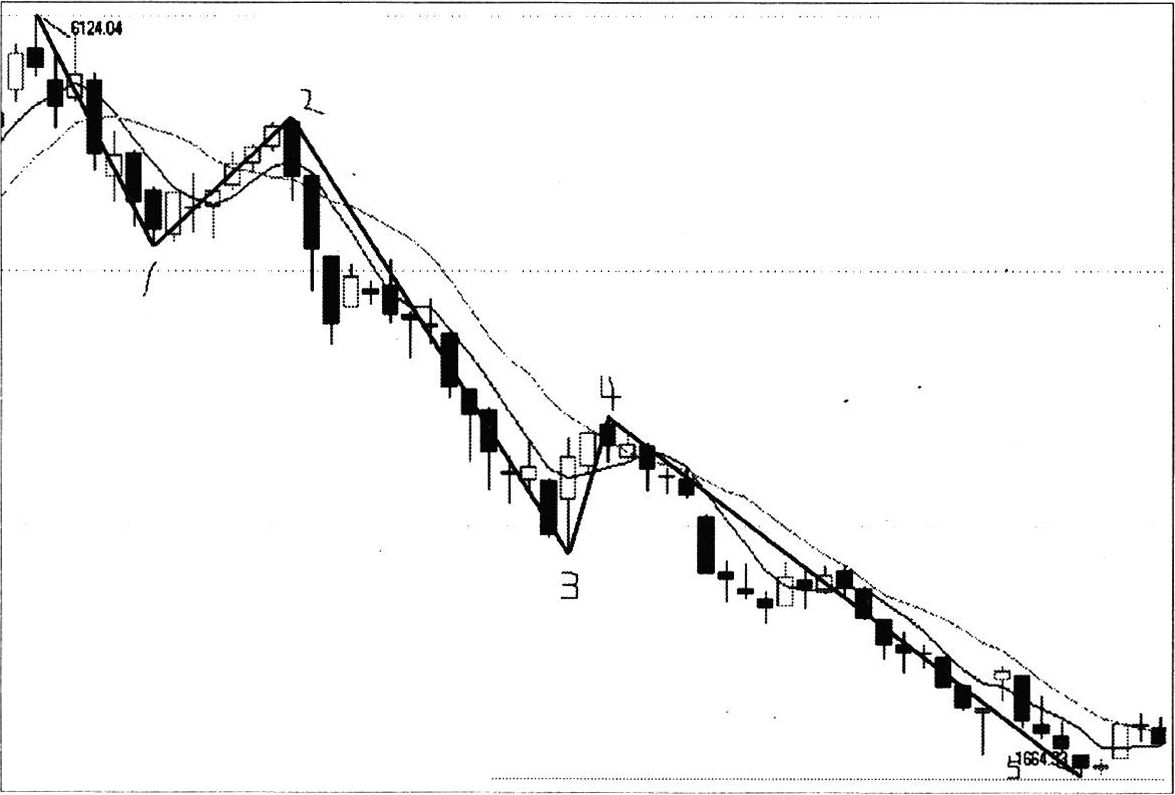
\includegraphics[width=0.88\linewidth]{images/9-1下跌五浪划分示意图.jpg}
\caption{下跌五浪划分示意图}\label{fig:forum-chart-1}
\end{figure}

由此我们可以将本轮下跌进行阶段性划分：3786点以上为高价区，该区域在大B浪反弹中将很难触及；2991点至3786点之间为中价区，该区域在大B浪反弹中将可能被触及；2991点之下为低价区，该区域在大B浪反弹中将很可能被收复。

我们可以从市场氛围中来验证以上波浪的划分是否正确。在1浪下跌中，中小投资者通常都在完美基本面信息的提振下认为熊市远远没有来临的可能；在3浪下跌中，中小投资者逐渐认同熊市来临的合理性，但仍旧认为股价相对于基本面被低估；在5浪下跌中，中小投资者在糟糕基本面信息的笼罩下认为股价相对基本面被高估。事实上，1浪下跌时的股民们等待股市再创新高；3浪下跌时的股民们等待一个不可能出现的大幅反弹来离场；5浪下跌时的股民们已经不再关注这个没有希望的市场了。

我们仍旧可以从图\ref{fig:forum-chart-2}中，将大A浪下跌的三个推进波继续划分出5个子浪。事实上，这样的划分同样非常完美。我们还可以发现，A5浪走出了明显的延长，下跌幅度要大于A3浪。

\begin{figure}[htbp]
\centering
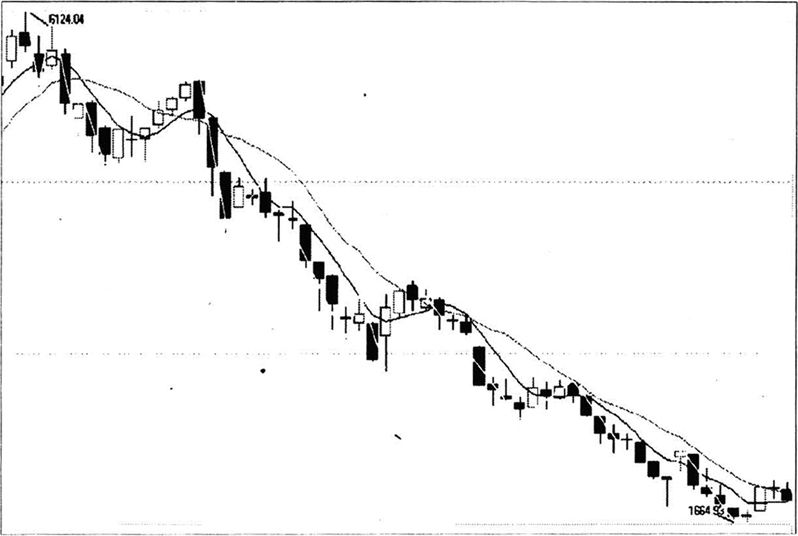
\includegraphics[width=0.88\linewidth]{images/9-2大A浪下跌子浪划分图.jpg}
\caption{大A浪下跌子浪划分图}\label{fig:forum-chart-2}
\end{figure}

\textbf{四浪的特性}

如果我们仔细从历史走势中进行观察，那么可以发现“四浪”通常与管理层的干预有关。例如，1996年的《人民日报》社论、2007年的5·30调整、2001年底暂停国有股减持形成的1515点至1776点反弹……有意思的是，A4浪和“A5浪的第4子浪”，都是因为降低印花税的利好而造就的。

四浪的特征还包括，其后大级别的调整行情将会触及四浪的波动范围，甚至对四浪的终点进行100％回调。上面列举的三个案例都符合这种特征，我就不详细解释了。这说明一个意思的规律：政策底（顶）从来都不会是真正的底部，但它们会对其后大级别的调整浪构成指引。也就是说，政策底（顶）不但距离最终的底部（顶部）不会太遥远，而且未来还会重返该区域。

我们似乎有理由认为：其后的大B浪反弹有可能达到2991点至3786点的区间，并且达到3786点的可能性最大。

\textbf{A5浪中的下降通道已经被突破}

图\ref{fig:forum-chart-3}中的两条白线为平行线，它们恰到好处地在1、2、3、4这四个点上重合。疲弱的五浪通常在突破三浪的终点后止步不前。突破低（高）点后并未继续前行是非常有违常理的事情，假突破对未来行情的提示作用，往往要大于真正突破的意义。

\begin{figure}[htbp]
\centering
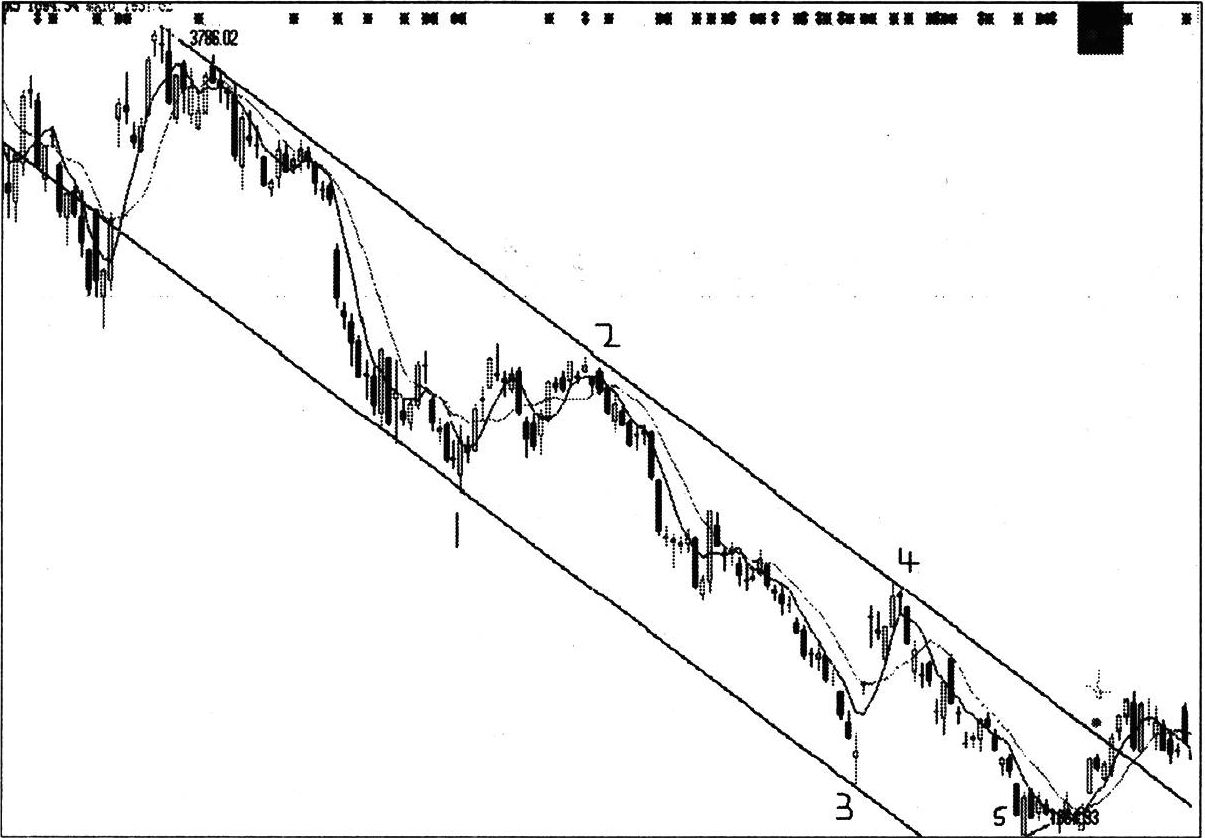
\includegraphics[width=0.88\linewidth]{images/9-3A5浪下降通道图.jpg}
\caption{A5浪下降通道图}\label{fig:forum-chart-3}
\end{figure}

从图\ref{fig:forum-chart-4}中我们可以清晰看出，上证指数在跌破1802点后就立即停止继续下跌。有意思的是，成交量有温和放大的趋势。大盘总是在即将破位之时，就被一股神秘的力量拉起。虽然这并非是失败的五浪，但的确是疲弱的五浪。熟悉波浪理论的人都应该知道，突破后立即折返的走势只可能发生在调整波中，或者推进波的第五子浪时。很显然，此次的情况是属于疲弱的五浪。而在此前的推动浪当中，任何被跌破的低点都不会被再次触及。事实上，大A浪下跌的目标点位为1500点，而某种力量阻止了最后150个点的下跌。

\begin{figure}[htbp]
\centering
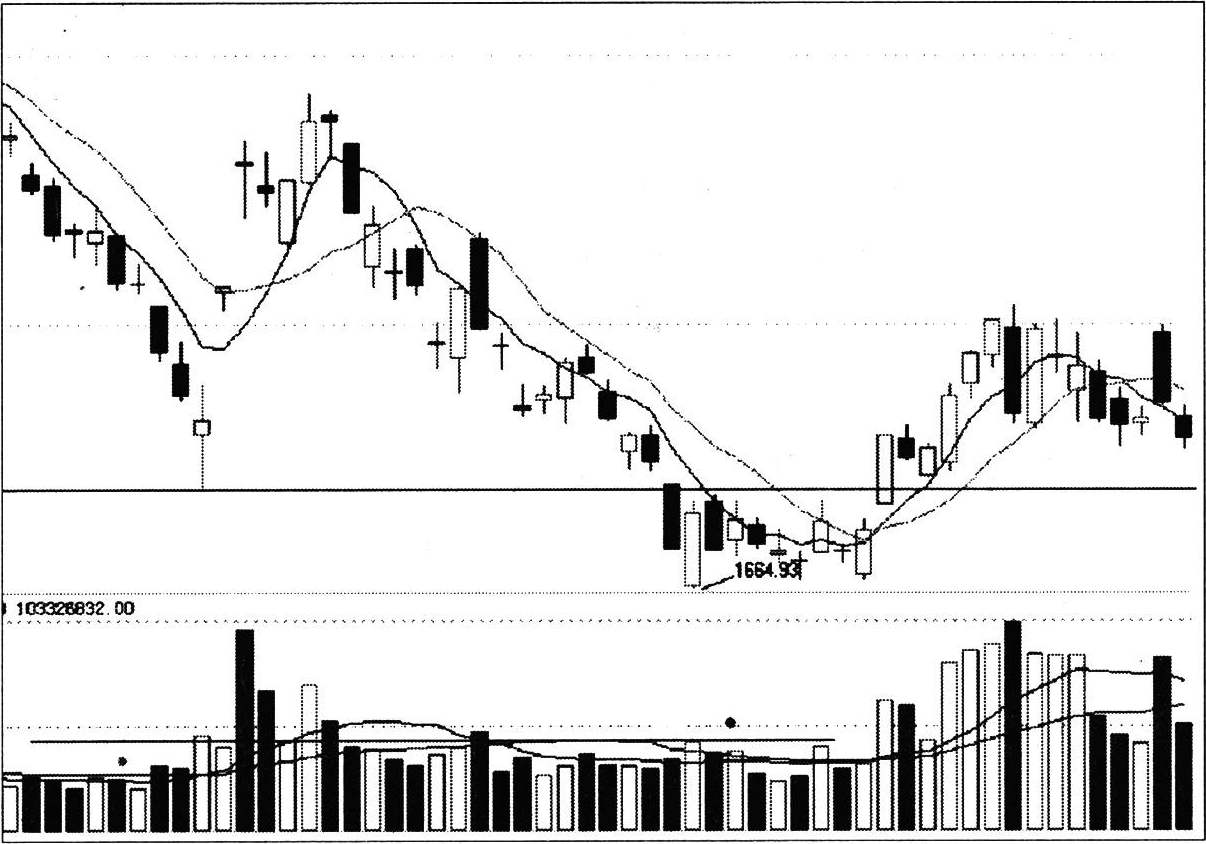
\includegraphics[width=0.88\linewidth]{images/9-4上证指数1802点走势.jpg}
\caption{上证指数1802点走势}\label{fig:forum-chart-4}
\end{figure}

\textbf{1500点的诱惑}

按照波浪理论和江恩理论的分析，我们将可以得出1500点为大A浪下跌终点的结论。表面上看，这种指出市场应该如何的说法有些大言不惭，但我们还是分析一下我的理由吧。

首先，1500点正好位于自998点为起点的重要江恩线。当然，没有人说得清楚江恩线绝对正确的画法，这使得该理论颇为神秘。但我们也并非毫无办法，而是可以从历史上（事后）找出重要的江恩线，并且用此线制作平行线。

从图\ref{fig:forum-chart-5}中我们可以清晰看出，对1994年325点至2001年2245点长达七年的大牛市形成支撑和阻力的江恩线。该线甚至一度阻止了2001年开始的A浪下跌，并且在其后的反弹中对股指构成阻力。最下方的白线同样是平行线，甚至该线阻止了998点后上证指数下跌至1067点的第二次探底。请注意，该点位目前正好位于1500点。

\begin{figure}[htbp]
\centering
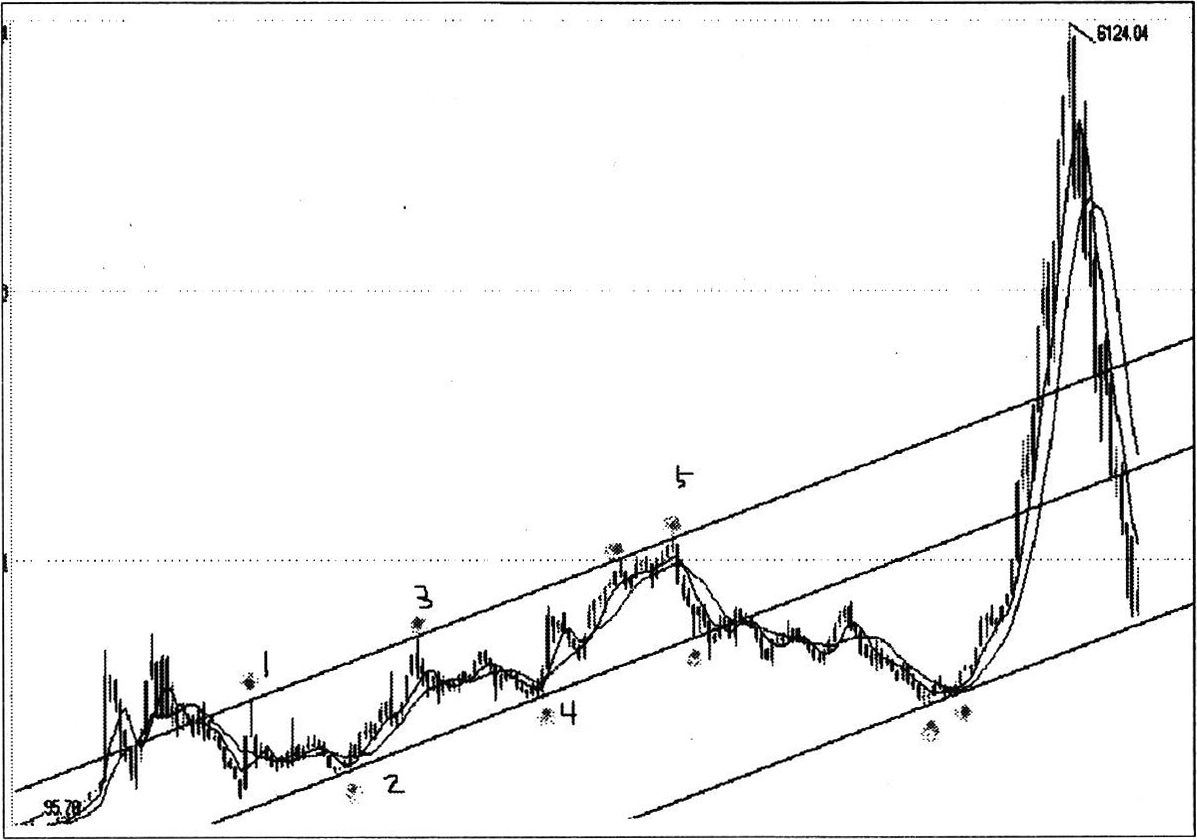
\includegraphics[width=0.88\linewidth]{images/9-5江恩线支撑阻力示意图.jpg}
\caption{江恩线支撑阻力示意图}\label{fig:forum-chart-5}
\end{figure}

其次，1500点正好对应2006年结束于1513点（1541点）的四浪回调。按照波浪理论的说法，四浪结束的终点会对其后大级别的调整行情构成吸引。这里有一个问题需要解释一下，我一直都说5·30调整为四浪调整，为什么1513点又成为了四浪的终点了呢？事实上，这非常简单。如果我们把998点至6124点的大牛市的上涨九浪视为大五浪发生了延长，那么1513点就是大四浪的终点，而5·30调整就为五浪4。

我们可以从图\ref{fig:forum-chart-6}中看出一个清晰的上涨9浪，但无法辨认究竟是哪一个浪发生了延长。5·30调整从市场的特征上来看，具有明显的四浪氛围。本轮熊市的A3浪正是在跌破5·30低点后不久结束的。但我们如果视为五浪发生延长，那么也与5·30调整的四浪特征不相矛盾。毕竟，它仍旧是大五浪中的第4子浪。

\begin{figure}[htbp]
\centering
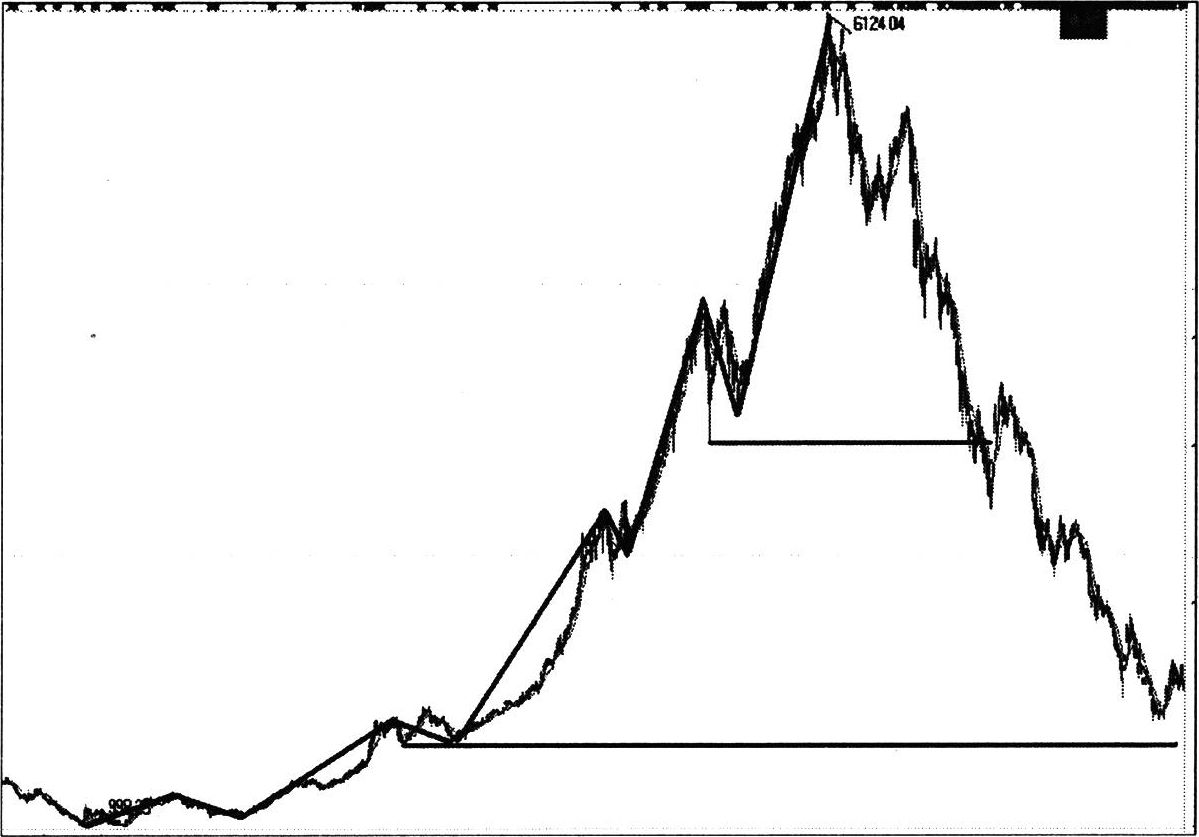
\includegraphics[width=0.88\linewidth]{images/9-6上证指数上涨九浪划分图.jpg}
\caption{上证指数上涨九浪划分图}\label{fig:forum-chart-6}
\end{figure}

我想很多朋友必然会存在疑问，四浪终点对未来的调整波构成吸引的规律是否真的存在呢？下面我们就在上证指数历史走势图中（图\ref{fig:forum-chart-7}）找出足够的案例来证实这一点。当然，例外也是存在的，1996年《人民日报》社论的底部就没有被其后的调整波跌破。但更加有意思的是，在深圳成分指数的走势图中，这个规律同样奏效。这一点大家可以在图\ref{fig:forum-chart-8}中发现。

\begin{figure}[htbp]
\centering
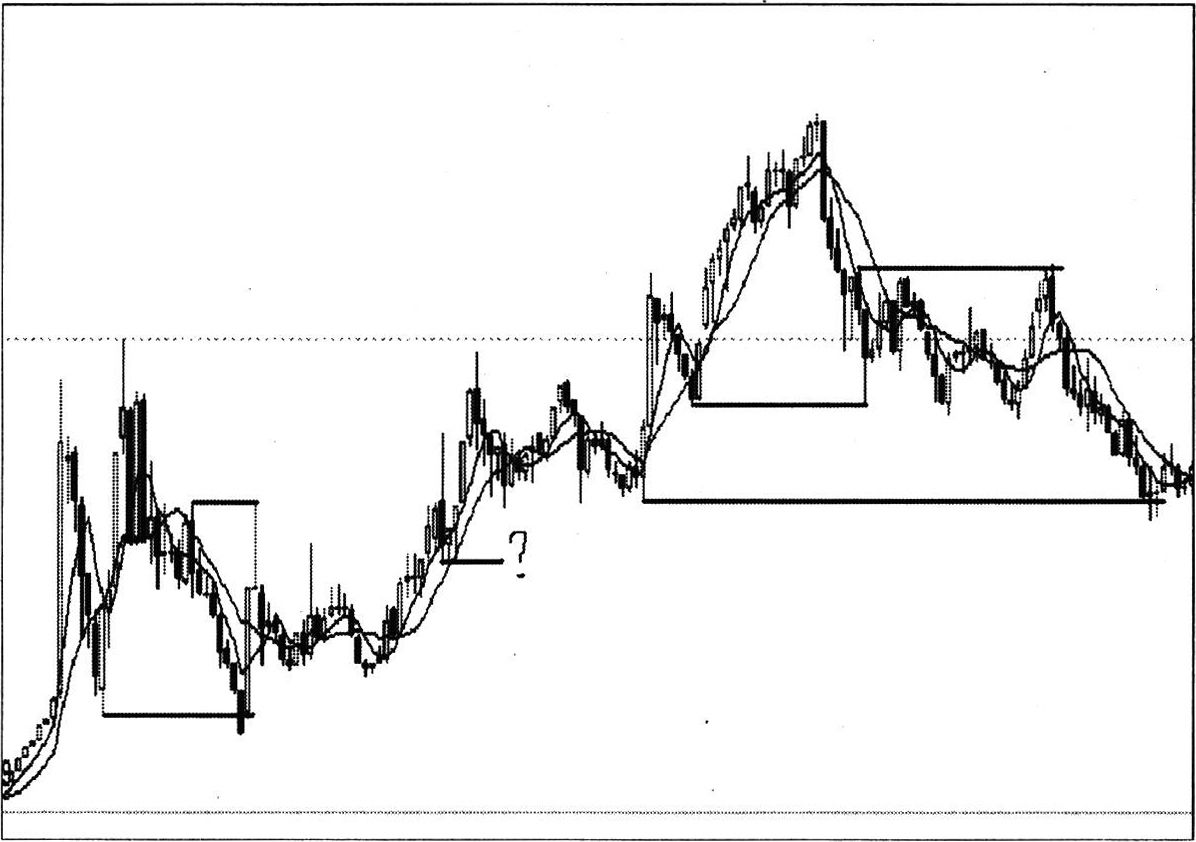
\includegraphics[width=0.88\linewidth]{images/9-7上证指数历史四浪终点示意图.jpg}
\caption{上证指数历史四浪终点示意图}\label{fig:forum-chart-7}
\end{figure}

\begin{figure}[htbp]
\centering
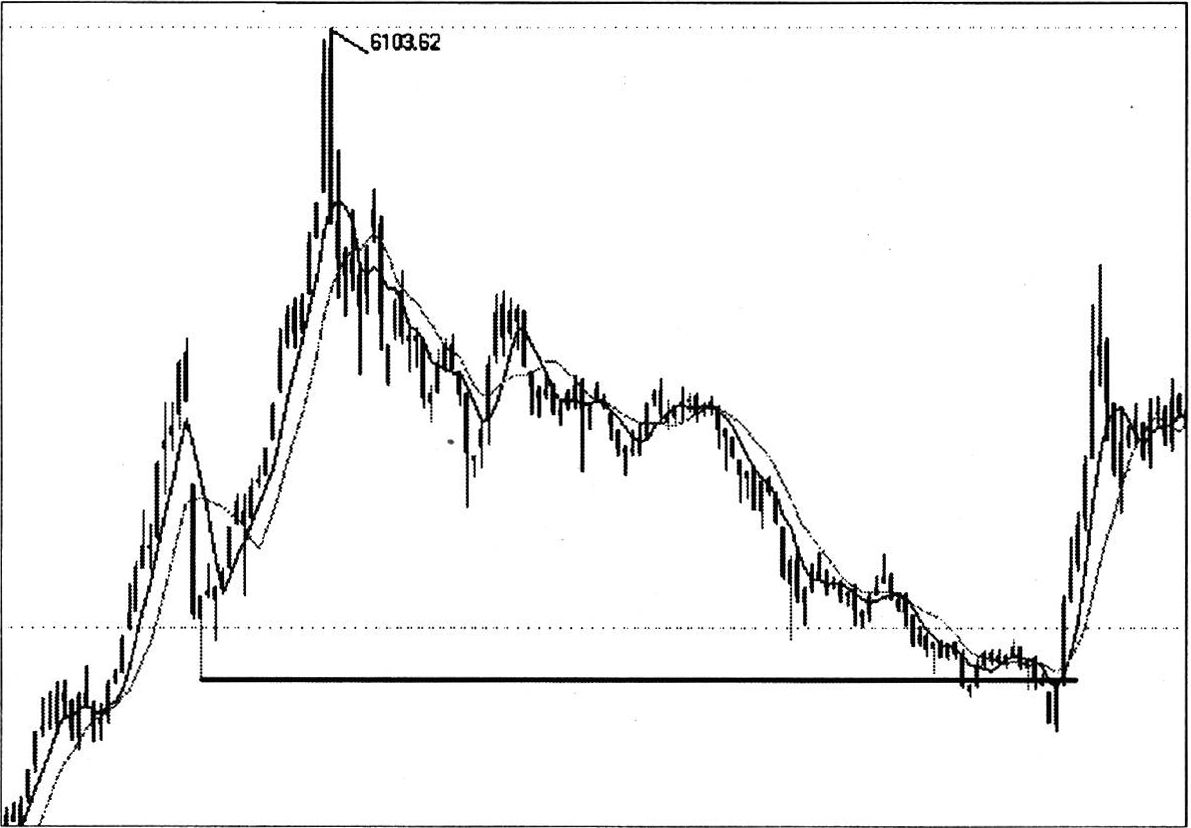
\includegraphics[width=0.88\linewidth]{images/9-8深圳成分指数四浪终点示意图.jpg}
\caption{深圳成分指数四浪终点示意图}\label{fig:forum-chart-8}
\end{figure}

最后，从黄金分割上来看，1500点也是完美的底部。如果我们将6124点至1500点进行黄金分割，那么A4浪的顶部3786点正好位于50％的中间位。如果我们将6124点至998点进行黄金分割，那么1500点也处于一个黄金分割位。更有意思的是，1500点与1997年的1510点的顶部位于一条水平线上，同时位于2245点至998点下跌的中间位附近。

\textbf{恐怖的基本面并不值得我们害怕}

很多论坛上的朋友向我指出：“未来根本就不存在任何的上涨因素，市场绝对不可能形成阶段性底部。”事实上，我目前同样也无法找出任何的向好因素，就像我在6000点的时候找不到利空因素一样。

我始终坚信，市场的力量大于经济环境的影响。是市场造就经济，而并非经济造就市场。我发现一个非常讽刺的现象：6100点的时候大众疯狂大喊股价便宜，并且遥望10000点；而1600点的时候大众恐慌大喊股价昂贵，并且遥望1000点。在我看来，市场上最有想象力的恐怕就是市场本身，它总会让参与者大跌眼镜。但是，当趋势能够激发出大众更加疯狂的想象力时，就距离趋势完结不远了。

当我打开美国黄豆三十年的历史走势图时，我发现了一个近乎完美的大箱体。有意思的是，当我打开美国黄豆的日线走势图时，我发现的却是连续不断的、近乎疯狂的上涨和下跌趋势。如此一来，我认为趋势和整理在不同尺度下是并不矛盾的事情。只要整理的尺度大于趋势的尺度一个数量级，它们将会被完美地统一。

有的时候我都觉得，被大众所热衷的高抛低吸本身并没有错误，而是大众在错误的尺度上进行高抛低吸。事实上，现在言底绝对是一种整理思维，但这却是月线图上的高抛低吸。我不得不承认，现在我使用的这些技术无法被运用于小级别的行情中。先不说微观走势凌乱，就是市场氛围的问题我也无法借鉴。我始终觉得波浪理论的“神”重于“形”。如果离开了市场氛围的阶段性分析的话，那么我无法使用波浪理论。事实上，月线图上的摆动类指标表现得非常出色，这说明在这个尺度下具有良好的整理特征。即使我们考虑到本体相似性，而将日线、甚至是分时图中的一根K线当做一个月，那么壮观的趋势行情恐怕要很多年才能出现一次。

事实上，当整理思维遇上了基本分析，就会出现一种可怕的灾难。市场的参与者并非是按照绝对的价格来评估高低，而是按照相对于基本面因素的相对价格来评估高低。这时市场信心理论就开始起作用，价格越上涨、基本面就会用更快的速度变好（或者说参与者就会越重视好消息而忽略坏消息），由此就觉得价格越来越便宜。所谓牛市，就是先上涨到让大众觉得非常昂贵，然后再上涨到让大众都觉得非常便宜。反之，熊市也是同样的道理。某证券公司在对2008年的展望中，预测上涨指数能够上涨到万点。我们无法用基本面数据来得出股票应该价值多少钱的结论。但如果将市场主流观点视为市场的价值所在，那么6000点的时候就是股价最为便宜的时候。

我们谈谈基本分析也无妨，结论仍旧是无需恐惧。如果某人不幸患上绝症，那么什么时候是最为恐怖的时候呢？我是说绝无好转的机会，并且会不断恶化。即使这样，答案也是在确诊的时候！事实上，全球金融危机并非绝症，但如今已经确诊！大家想想看，未来经济会如何发展呢？是否最为恐怖的阶段已经过去了呢？对于中国股市就更加有意思了，大幅下跌后的低位，利空是完全可以当做利好来理解的。如果真的存在那个“它”（无形之手、市场主力），同时“它”也有能力将股指打压至千点以下，但是大家想想看，如果未来市场不存在更加恐怖的基本面信息，“它”是否能够完成战略性建仓呢？《股票做手回忆录》讲述了这样一个故事：主人公持有巨大的棉花头寸，并没有兑现的计划。但因为报纸刊登了棉花被垄断的利好而刺激出强大买盘的时候，主人公立刻决定平仓出局。想想看，全球金融危机的爆发，是否也让大资金在没有买入计划的情况下被迫买入呢？事实上，大资金控制价格并非困难，困难的是找到对手盘。全球金融危机都已经是百年一遇了，那么未来还会有更加新鲜的事情发生吗？

全球金融危机不但使得GDP的增速出现大幅下滑，同时也会使得CPI和利率大幅度降低。我们不妨设想一下，能够左右股价高低的三个因素在于业绩、利率、通胀率。如果这三个指标同时出现三分之二的下跌，那么是否会相互抵消对于股价的影响呢？事实上，本轮熊市初期的下跌，并非是因为对业绩问题的担忧，而是对于高通胀、高利率的恐惧。

对于大小非的问题来说，我们也完全没有过分担忧的必要。我不否认，自今年12月至明年5月是大小非的解禁高峰。但一个显而易见的问题都被大家忽略了，小非的减持高峰早已过去！按照减持规则来看，自支付对价换取流通权后，持股低于5％的股东在一年后就可以解禁。事实上，股权分置的问题在一年前就基本上已经解决完毕。

我们可以将小非理解为个人财富。如果我突然暴富的话，那么可能就会买名车豪宅。同时，我们也可以将大非理解为社会财富，他们是被记录在某某公司名下的财产。企业是无法进行疯狂消费的，而私营企业的老板根本不用解禁股票释放出的资金，就能享受他们可以享受的一切。想想看，他们如果真的抛出了持股，那么他们的钱会流向何处？难道是存入银行吗？要知道现在利率低得可怜！难道是扩大生产吗？要知道现在的经济危机早已使得生产过剩。如果是2005年以前，这种情况或许会发生。因为那时股市低迷，而产业资本却是非常赚钱的。事实上，实体经济和虚拟经济在宏观上是趋同的，但在微观上却是明显的跷跷板，因为产业资本和金融资本在进行争夺。日本经济泡沫是如何产生的呢？不就是实体经济不赚钱了，大量资金流向虚拟的资本市场吗？

退一万步说，大非绝对是市场上的强势群体，他们真的不会贪得无厌而贱卖捡来的黄金吗？如果他们不是贪得无厌，那么也不配成为做大做强的大非！大非的解禁是一种不用费时费力进行收集，就能够实现的筹码集中。想想看，2000年的股市能够将转配股上市当做题材来炒作，那么现在为什么就不能将大非解禁当做题材操作呢？回顾过去十多年的炒股做经历，我不得不感叹：市场真实的发展，通常与大众的思维截然相反。如果不是为了反驳大众的观点，那么我是不会试图解释市场的。奢望找到市场的逻辑，是这个世界上最愚蠢的事情！

最后，我们再来对未来的行情进行一下展望吧。很多交易大师都认为，预测市场将会发生什么走势并不是最困难的事情，最困难的是预测这种走势会在什么时候发生。波浪理论也告诉我们同样的道理：波浪的形态、比例都不是最难预测的东西，最难预测的恰恰是波浪运行需要的时间尺度。下面的观点，本人尽量回避关于时间的问题，而着重谈谈未来市场可能呈现的波动特征。

\textbf{第一，大熊市远远没有完结的可能，大牛市的到来还是非常遥远的事情。}很显然，大牛市应该是在市场抛压最小的时候才会到来。那么，什么是市场抛压最小的时候呢？获利抛压是市场永远都不可能摆脱的压力。除此之外，抛压主要体现在解套抛压，这是由市场参与者的本能所决定的。

我们可以想象，当市场上一部分股票已经创出新高，自然就不存在解套抛压；一部分股票大幅下挫而远离此前的成交密集区，大幅上涨也不会立即释放解套抛压；一部分股票在低位长时间横盘筑底使得筹码经过充分的换手，被拉低的持股成本也可以解决解套抛压的问题。我们可以从历史上清晰地发现：无论是1999年的1048点还是2005年的998点，市场都出现了这种抛压最小的内部结构。

事实上，目前市场上的全部个股具有明显的趋同性，都处于大幅暴跌后的状态。如果中国股市就此走牛，那么未来将会在同一时点上面对巨大的解套抛压。很显然，牛市的真正到来需要未来长时间的个股走势分化来酝酿最终的底部。

按照波浪理论的说法，一波清晰的五浪下跌，只可能是更大级别熊市的一条腿。按照本人的“市场层次理论”，此前的下跌属于所有股票一致性下跌的绝对熊市；此后的上涨属于酝酿长期热点的熊市换档；最后只有在分化下跌（部分股票暴跌、部分股票抗跌）的相对熊市走完后牛市才能够到来。

\textbf{第二，分化是未来很长时间市场的明显特征，}“轻大盘、重个股”是明智的选择。如果按照“股市层次理论”的说法：市场上的一部分股票在1665点就已经走完了熊市的路程，这类股票现在已经步入牛市；同时市场上还有一部分股票仍旧会走出大幅下跌的走势，这类股票的熊途才刚刚走完一半。事实上，未来熊市中的强势股就是下一轮牛市的主流热点，这种大尺度的热点至少会持续三到五年的时间。那么，什么样的股票是未来市场上的强势股呢？

我不相信，市场上存在一种可以选出某一特定黑马的可量化技术，而我们所能做的只不过是在宏观上寻找未来热点的特性。按照最宏观的分类方法，我们可以将全部股票分为“蓝筹股”和“概念股”两类。所谓蓝筹股就是，盘子大、业绩好、以基金持有为主的一些股票；而所谓概念股就是，盘子小、业绩差、以游资持有为主的一些股票。

虽然我不能回答未来哪些股票能够成为黑马这一问题，但我却可以尝试猜测一下未来哪类股票可能成为热点。我的答案很简单，未来的中国股市将是概念股的天下！这样一来，我们选股的主旋律就将围绕着“价格低一点、盘子小一点、业绩差一点、基金少一点”的四点原则。反之，就是我们应该回避的股票。没错，业绩好的股票也是我们应该回避的！！我相信，没有人看到这样的观点时不会感到惊讶。要知道，这无疑是在同市场上几乎所有的权威在唱反调。下面我就解释一下我的道理吧。

股票的炒作需要什么？事实上，根本就不需要什么良好的业绩，甚至不需要丰厚的红利。在过去的大牛市中，持股者获得的红利收益相对于股价波动带来的资本利得根本就是九牛一毛。那么，股票炒作最需要的是什么呢？很简单，是一个可以被大众接受的借口！记得，1998年最为疯狂的一些股票，现在都已经退市。比如，托普软件、科利华、北大车行等。微观上的大幅上涨与宏观上的破产，并不是一件矛盾的事情。

要知道，我们正处于百年一遇的世界金融危机当中，未来上市公司的业绩注定会出现下滑。如果说，未来上市公司的业绩注定不会很好，那么股票的炒作必须绕开业绩的尴尬。如果市场主力不能改变参与者头脑中对于业绩与股价呈现绝对相关性的偏见，那么，任何炒作行为都是不会成功的！

当现实已经变得一团糟时，重要的就是对于未来的希望。“市盈率、估值水平、价值投资”等词语，未来会显得非常落伍和不合时宜。经济萧条的另一层含义还在于，市场上能够流动的资金会显得非常有限。股票市场除了全线下跌的绝对熊市以外，资本的逐利本性总会使得一些股票大幅上涨。区别在于，绝对牛市时资金可以充裕到将所有的股票炒热。甚至在货币泛滥的牛市中，小盘股都无法容纳庞大的主力资金。当市场上的资金匮乏时，主力资金的唯一选择就是“缩容”炒作。这就好像1997年以后的中国邮市。邮局疯狂发行邮票而使得市场上的邮票泛滥，最终使得邮票的面值都无法支撑住价格的下跌。有意思的是，此后虽然邮票价格步入了永不见终点的熊途，但像猴票这样的稀缺品种却以越来越快的速度上涨。我相信，在未来的中国股市上，稀有的资金也会绕开泛滥的筹码，而“扎堆儿”在稀少的、没有可比性的品种上。很显然，虚拟的希望是没有可比性的，而有形的基本面数据就绝对不具有这样的特性。记得1999年初的中国股市，游资甚至绕开所有的股票，扎堆在数量不多的小盘基金中，将其炒作到净资产的数倍！

在我看来，中国股市未来的走势很可能类似于1998年的股票市场。老股民一定会记得那个疯狂博傻的年代，而新股民就会显得非常吃亏。有意思的是，博傻游戏中最后的傻子，通常都是在初期最理智和清醒的那些人。觉得市场愚蠢的人，才是市场中最愚蠢的人。1998年的经济环境处于东南亚货币危机当中，而现在的经济环境处于全球经济危机当中。或许，相同的原因就能够产生相近的结果。当年，实体经济的破灭使美元大幅度走高、大宗商品期货大幅下跌、纳斯达克指数明显强于道琼斯指数……直到2001年实体经济逐渐恢复时，美元才不断走低、大宗商品期货大幅上涨、道琼斯指数崛起同时纳斯达克市场破灭。

某交易大师说过：“上一轮牛市的热点，如果持续到本轮牛市中，那将是非常不同寻常的事情。”如果我们仔细研究中国股市历史上的热点分布，那么也是可以得出类似结论的。事实上，热点板块经常会跨越持续时间只有6个月左右的中期熊市，但从来没有什么热点能够跨越长期牛熊循环。我所经历过的长期牛市只有三次：1996年至1997年的长期牛市；1999年至2001年的长期牛市；2005年至2007年的长期牛市。在这三轮长期牛市中，它们各自最热的领头羊分别为：四川长虹、亿安科技（ST宝丽华）、沪东重机（中国船舶）。有意思的是：四川长虹和青岛海尔等家电股虽然在1996年以前就业绩优良，但它们从来就不上涨，甚至被大家戏称为伤心概念股；1997年四川长虹高高在上时，未来的黑马亿安科技只有区区的几元钱；而当2001年亿安科技跨越百元大关时，未来的龙头沪东重机也只有区区的几元钱。那么，未来真正的超级黑马，现在是否也只有区区的几元钱呢？在我看来，大幅上涨的好股票并不可怕，但大幅上涨后出现下跌的股票才是最可怕的！相信我，好的股票是从来都不应该下跌的。我们可以从历史上的大牛股中发现，它们经常都是很多年都不会出现下跌的，而当它们真的开始下跌后就会一蹶不振。《股市倍增术》中说过这样一种观点：大幅炒作过N倍的股票，我们N年不碰。当然，这样的观点并不完全正确，应该是大幅炒作后出现大幅下跌的股票N年不碰。一轮长期牛市的到来，说明市场中的主流热点必须另起炉灶。

熟悉本人“股市层次理论”的人应该知道我对于股市阶段的划分。如果我们仔细观察相对牛市中不同类型股票的走势，那么就能够轻松找到下一轮牛市的热点概念。1996年12月856点至1510点的中期牛市、1999年12月1341点至2245点的中期牛市、2007年6月3404点至6124点的中期牛市都属于相对牛市。相对牛市的主要特点在于，市场上一类股票反复走强，而另一类股票出现明显抗涨，甚至无法创出绝对牛市的新高。事实上，6124点时很多股票都无法创出5·30调整时的高点。我的结论是：相对牛市中大幅上涨的股票，未来通常都会一蹶不振；而相对牛市中疲弱抗涨的股票，未来通常都会成为主流热点。我相信，未来股市中的热点将会是5·30调整后热点的对称版。让我们回忆一下，那个年代什么样的股票表现最好呢？业绩好一点、盘子大一点、基金多一点、价位高一点，对吗？

在6124点的大顶构筑时，我正巧在银行的大厅内上班。我亲眼看到了大量不明真相的老头儿、老太太疯狂买入基金。事实上，他们是社会上最为弱势的群体。这也说明，基金最为疯狂的年代已经过去。基金未来的销售将会越来越困难，这是很明显的事情。另外我很了解弱势群体的思维模式，他们几乎是一个模子刻出来的。只要他们的投资不能够盈利，那么他们就不会赎回基金。同时，当他们真的能够解套时，那么就会用最快的速度将基金赎回。如果基金重仓股的价格大幅上涨，那么将会遇到赎回浪潮的抛压。谁会当解放军呢？虽然我很善良、很同情弱势群体，但仍旧觉得应该让他们品尝一下轻信别人的代价。从另一个角度上来讲，基金公司的盈利模式在于管理费，他们也不愿意看到基金规模大幅缩水。难道还不够清楚吗？谁是熊市另一条腿的做空动力不是一目了然了吗？

这里我提醒大家注意一点：虽然短时间内就会推出融资融券的业务，但大家融资买入蓝筹股时一定要慎重。更重要的是，千万不要去沽空在熊市中拉升过一波，并且股价相对于基本面明显被高估的股票。

\textbf{第三，未来行情的走势。}前面我们已经将未来的上涨定义为熊市中的大B浪反弹，或者是熊市换档。调整浪的特性就注定了未来市场的走势不会呈现简单的特征。调整浪都是非常复杂的、震荡噪声很大、趋势感不明朗。当然，大级别的B浪反弹在幅度上很可能不会逊色于1999年的5·19行情。这里我提醒使用趋势跟踪系统的交易者，对未来系统会面对的噪声水平做好心理准备。

我不知道市场能否被预测，但我非常肯定对于获利而言，正确的预测的确不是必需的。我经常在看不懂行情、甚至是看错行情的情况下获利。即使我靠预测进行交易，那么其中也必然会使用“如果……那么……”的思维方式。或者说，我会随着行情的发展，而不断调整本人对市场的预测。自然，过多谈论市场走势的意义，远远不如谈论市场特性更加重要。

简单说，我觉得未来的行情很可能会分两步走。其中，第一步属于超跌反弹；而第二步的热点股票不排除创出6124点新高的可能。对于具体的指数而言，2009年的波动区间很可能在1700点至3800点之间运行。如果1665点成为大A浪下跌的终点，那么大B浪很可能会达到3000点到3800点之间。甚至，第一步会达到3000点，而第二步会达到3800点。

我不想对未来的顶部谈论过多，因为买入的技术是“并且”的关系，而卖出的技术是“或者”的关系。当股指出现一波明显的上涨后，单单跌破止损点这一个因素就绝对能够让我们全线离场。

\textbf{结束语}

我相信，在网络上与大家分享我个人这种离经叛道的思路，应该是一件受到很大压力的事情。甚至，很多人听到这种荒唐的言论都会非常的有气，就像我听到主流媒体的观点时一样生气。总之，不管怎么说，结果都是不重要的事情。我从来都不希望本人的观点能够帮助大家获利，真正重要的是我的思维方式。如果我这种荒唐的想法最终被市场证明是正确的，那么我希望的也只不过是大家能够反思一下头脑中一些理所应当的信念。

除非你自己也能够得到与我相似的观点，否则我是不建议任何人买入股票的。无论最终的结果会是如何，一个不能够捍卫自己信念、不能独立思考、不能为自己负责的交易者，根本就与那些6000点大买“没有风险”的开放式基金的老头儿、老太太没有任何区别。这样的人，只会成为强者食物链中的羔羊。

没有人会不犯错，即使我的犯错率超过60％，我仍旧还是可以获利。我不希望这篇文章干扰到任何人，更不希望这篇文章被大家误认为是一篇预测性的文章。我很久以前就希望同大家谈谈波浪理论，但谈论过去行情的照本宣科是没有任何意义的。要知道，数历史行情的波浪，是永远都不会有错误的。

本来我还想同大家分享我的持股，但考虑到“北化事件”还是决定不要误导大家。到目前为止，我持有股票的市值为103万，持有的股数为28万股，平均股价为3.68元。本人所持有的10只股票价格都位于3元到5元之间。其中，3只为中小板股票、8只为券商重仓股、2只业绩亏损股、7只股票净资产低于2元。

\subsection{2008年交易回忆录（2009.01.09）}

似乎我从来没有写过叙事性的文章，今天我尝试对已经过去的2008年进行一次回顾。希望大家和我一样都能够从我的经历中，获得对自己有益的经验。

\textbf{走势分化、资金实现软着陆（农历新年之前）}

记得2007年的头一个交易日，资金在大幅增长后出现了单日6位数的巨大亏损。过重的仓位使我仓惶而逃，这也使我在豆油上丢掉了极其庞大的利润。要知道，整个2007年豆油都是在简单地不断上涨！事后看来，在其后的2008年里，豆油出现了更加壮观的大幅上涨行情。或许，连续不间断跟踪是永不丢掉跟踪位置的唯一办法。但与此同时也会出现一个新问题：当趋势完结的时候，资金权益会出现比较大幅度的回撤。如果说在此前的趋势中过度依赖浮动盈利加仓，那么价格折返带来的资金回撤就有可能是毁灭性的。这也是我暂不依赖浮盈加仓的道理，我不想丢掉在市场中的长期位置。

有意思的是，从2007年8月到2008年初，本人的资金权益同样出现了接近100％的巨大升幅。那么，坚持系统的机械操作是否会再次让我经历庞大的资金回撤，甚至是出现可怕的硬着陆呢？每当市场出现壮观的趋势时，我都能够获取庞大的利润。但这种获利的过程通常并不会让我感到兴奋，因为我知道其后会有永远都不可能摆脱的资金大幅度回撤。资金权益增长是以扩大跟踪乖离率为代价的，而乖离率的扩大意味着潜在风险的扩大。

2008年初，并没有出现我所担心的硬着陆，而是资金在历史最高位横向震荡使乖离率被彻底挤出。我将在农产品多头市场所获取的利润，投入到工业品的空头头寸持仓之上。很幸运，工业品与农产品的分化显然让我获取了更多的利润，而后又让我的资金权益出现了软着陆。

这是一个有创意的方案，用趋势中的浮动盈利投入新的市场，用来对冲庞大的乖离率风险（价格折返风险）。在一年以后的今天，我同样是将在金融危机中大举做空商品期货赚来的利润，投入到股票市场进行风险对冲。到目前为止，这种操作还在继续之中，效果还不能作出最后的评价。在我看来，这种利用浮动盈利来对冲乖离风险的办法很可能是绝佳的。

当期货头寸从全线同方向持仓，转变为大面积多空对持时，我就已经可以笑着说，我的双脚已经平安着陆了。接下来大家将会看到，飞得更高也会摔得更狠的案例。在我们尚未双脚着地以前，是不应该轻言胜利的。

\textbf{多头陷阱使资金权益大幅波动（1月底至3月底）}

本以为资金软着陆后，能够出现很长一段时间的平静期。但阴历年过后，各个期货品种都开始出现明显的上涨行情。一个个品种在短时间内集中发出买入信号……难道新一轮的资金增长开始了吗？看着这种罕见的启动力度和市场广度（全部品种一致上涨），让我不得不联想到这是一条我从未见过的大鱼！

我已经别无选择地陆续将空头持仓翻多，最终出现了全线持多的局面。“帝国指数”从1月28日的53.14点快速上涨至3月4日的76.31点，甚至在3月4日盘中见到过82点以上的高位。这是历史性的突破，我从来没有见过这么多钱！我深信这只是庞大财富的开始，因为中期行情至少会持续三个月。庞大的仓位可以使我赚取上百万的利润，这是顺理成章的事情。要知道，这是我从未见过的市场广度，就连平时非常呆滞的棉花和铝都出现了大幅上涨。事后看来，这种市场广度可以与国庆节后的金融危机时期相媲美。

就在这时，兴奋得几乎飞起来的我作出了一个荒唐的决定：辞去工作，专职交易！客观地说，辞职的想法早在这之前就已经存在，而交易上的起色让我更加坚定辞职是对的。我之所以使用“荒唐”这个词，并非是因为这个决定，而是因为我的动机。现在我已经可以确定地说：即使那次真的出现壮观的中期牛市，让我获取超过百万的净利润，那么仍旧有太多的问题是我没有想到的，专职交易的成本并非只有钱这么简单。讽刺的是，在我辞职后的2周时间内亏损了38万，一辆国产宝马没有了！此后，我在从未有过的“囊中羞涩”中度过了艰苦的半年，每个月的零花钱只有500元。或许，那时并不存在心理压力，也没有孤独的感觉。因为极度贫穷的我，哪里还有资格考虑这些抽象的东西呢？

言归正传，在我极度兴奋中，市场出现了戏剧性的一幕：开盘不久大量的品种已经封死或接近涨停板，而豆油也出现了连续第N个涨停板。我之所以印象深刻，是因为那天是我最后一天上班。我在10点15分第一节收盘后才懒洋洋地去了一趟银行，当我到银行打开笔记本电脑时发现：豆油居然从涨停直接打到跌停板，大量的品种跟着跳水……

这是一种很奇妙的感觉：看着价格跳水，我居然完全无能为力！基本上市场根本就没有任何的反复，而出现了义无反顾的下跌。起初，我还可以认为这只不过是一次强洗盘，但下跌的态势却越来越凶猛。天哪，期货的亏损速度居然会这么快！我将自己封闭在屋子中，不吃不喝、甚至不想见人。哎，一辆国产宝马对于有钱人来说恐怕不算什么，但对于我这样的穷人就是大过天的事情。

我已经不再对中期牛市抱有任何幻想了，但我也不能够逃跑！听说过量子理论的测不准原理吗？一个微观粒子的某些物理量（位置和动量、时间和能量等），不可能同时具有确定的数值，其中一个量越确定，另一个量的不确定程度就越大。其实市场也具有相同的特征，趋势和价位这两种特征，其中一个量越确定，另一个量的不确定程度就越大。虽然暴跌的持续，让我深信上涨趋势已经完结了！与此同时，我对于价位的问题就非常不确定：市场会出现反弹吗？

说到这里有些人就会不理解了：有没有反弹同快速止损并不矛盾呀，你不是求势不求价吗？这种说法无疑是正确的，一个主观型交易者完全可以在趋势完结时不管价格地离场，甚至这完全是必须的纪律。但对于系统化交易的我来说，脱离系统等于背弃信仰，这甚至有种类似于失去道德的压力。我很清楚，离开了信念，得到的东西也会最终失去。

前面提到了连续N个涨停板的豆油，而我的第一桶金就是用近乎疯狂的仓位在豆油上获取的。遗憾的是，在2007年初，我将豆油的多头头寸丢掉了！我的确在豆油发出卖出信号的时候离场，但其后的买入信号我却没有参与。我很难估计因为丢失这个信号的损失。根据混沌理论，初始值的一个细小变动，就可以让结果出现天大的变动。我不会去算我在豆油上相对于系统少赚了多少钱，而是会去算让我丢掉的资金增长多大幅度。事实上，这让我失去了将资金增长几倍的机会。假设后期的操作完全不变，那么我丧失了至少500万以上的纯利！其实呢，我如果能够规避最近三年来的两三个错误，那么我的资金将会早已过千万！

我说这些是告诉大家，我绝不允许自己再丢掉市场上的位置！请注意，不是趋势中的位置，而是市场上的位置。我们假设，豆油在2007年并没有暴涨，那么我就没有丢掉在趋势中的位置，对吗？但如果豆油其后出现了暴跌，而我并没有参与空头，那么这就叫做丢掉在市场上的位置。一个出色的趋势交易者，必定会有这样的目标：只要市场有趋势行情，那么就必须赚取属于我们的利润。这意味着什么呢？这意味着我必须让我自己的资金永远在市场，只有这样我才能够保证实现自己的目标。我想说的是：我在市场上必须做到永远持仓，我能够做的只是调整方向：非多即空！

明白我的意思吗？即使我看出上涨趋势已经完结，但我也不能够逃跑。如果我不能够由多翻空，那么我就只能够持有多头头寸。我的决定无疑是正确的！我在半年后的金融危机中赚取了不少的利润，功劳在于我没有丢掉市场上的位置。没有人能够保证看出金融危机的到来，我也不能！但我能够保证，我一定会在金融危机中获利，只要金融危机到来的话。

系统告诉我，我应该等待卖出信号，并且在那时由多翻空。问题是前期的快速上涨，使得乖离率过大，而两条均线也处于发散状态。这说明当趋势起飞以后，系统会接受和容忍更大的波动率。即使价格跌破中期跟踪均线，但我仍旧需要等待短期过滤均线与其交叉。我很清楚，这是市场对我恰到好处的打击，也是我可能出现最为糟糕的局面。很简单，让我大亏的前提必须是让我先赚钱。如果市场没有让我赚钱，那么价格轻微的反向波动就会使我转换持仓方向。赚钱是必须的，关键是让我赚了多少？如果趋势能够持续更长的时间，那么利润就绝对可以抵消这种大亏。如果趋势能够持续更短的时间，那么过小的利润也只能够引发不大的亏损。

直到今天，我还有一种“起飞时的恐惧”。这就像航天器的发射，点火后几分钟是最危险的。挑战者号航天飞机不就是在这段时间失事的吗？点火以后，一切都将不可逆转，谁都不能够让其停下来……我可以绘制一种趋势起飞后的“最大潜在风险曲线”：随着均线的发散以及跟踪乖离的增加，甚至包括持仓方向的集中（大的趋势必然有大的市场广度），最大潜在风险曲线会快速走高。当然，与此同时，资金权益曲线也会出现明显的增长。问题在于，最大潜在风险曲线的增长速度要快于真实的资金权益曲线的增长！好在，最大潜在风险曲线的增长具有衰竭性。当起飞上升到一定高度后，就会出现走横的局面，而不会进一步增高（这种高度与我们采用的跟踪尺度参数有关）。事实上，资金曲线的上涨是不会衰竭的，当利润数量超过最大潜在风险值后，我们就处于“赚多还是赚少”的安全地带。如果趋势能够继续，那么最大潜在风险曲线也不会出现下跌。趋势结束后的资金回撤期是我们永远无法摆脱的问题。当趋势结束的时候，最大潜在风险曲线会随着资金曲线一起走低，而这可以通过两种方式实现。如果市场出现分化、或者是横向震荡来挤出乖离率，那么就会出现资金回撤幅度不大的软着陆；而如果市场集中出现转折，形成尖尖的转折点，那么就会出现很大资金回撤幅度的硬着陆。有人可能会问：最大潜在风险曲线能否用数学来进行可量化的表述呢？我没有办法计算精确数值，因为这涉及时间和幅度两个问题，但我也可以勉强推出一个表述公式：潜在最大风险=跟踪乖离率+两条均线的乖离率×某个常数。

我从这次多头陷阱事件中学到了很多的东西，也让我第一次感受到了暴仓的恐惧。上面说了这么多，只是想说明系统是我的信仰，而我是不能够背弃它的。即使翻空是肯定的，那么我也需要用信号来确定翻空的时间和点位。毕竟，我不能够排除反弹的可能，更不想遭受提前做空而出现反弹的计划外亏损。

但市场是现实的，我的结算准备金已经趋于枯竭！我很庆幸自己做对了两件事情：第一，我没有利用浮动盈利加仓；第二，我已经建立了资金储备制度。事实上，我的期货账户已经暴仓了，而我是利用资金储备解决了问题。由于交易所对于保证金的提高，即使我将全部资金储备都用上，那么我的风险度还是在最后一天超过100％。要知道，我在两周前的仓位只有40％（将储备资金计算在内）。我想我无法用语言来形容这种恐怖：暴仓的恐怖！很多人可能会轻蔑地说：“做期货的人有谁没有暴仓过呢？”相信我，这是不一样的！如果你将全部家产投入到期货市场，那么暴仓就绝对不是一个可以轻松的词汇。同样的道理，一年100％的收益率与家产翻番也不是相同的概念。更可怕的是，股票亏损是可以逃避的，而期货的亏损是不可以逃避的。即使真的要不计代价地砍仓，那么也必须由我自己下手。或许结果是一样的，但责任上的意义是不同的。

这时我已经必须要作出选择，而选择只有两种：第一，脱离系统进行避险操作；第二，等比例缩减持仓数量。或许还有第三种方法，那就是放任自流。事实上，我在等比例缩减仓位三分之一的那天，几乎就是我资金权益的最低点，帝国指数的44.62点。虽然风险度超过100％但也不足110％，何况这还是在大幅提高保证金率后的情况。当市场恢复平静后，保证金率就会出现下降。事后从结果上看来，第三种选择会带来最好的效果。仓位应该不会被强平（强平需要到第二天），而我其后的利润也会增加三分之一。

我必须作出选择！我来到市场上是为了获利，而系统是我获利的基础。我当时对我老妈说：“无论承受多大的代价，我都不能够丢掉自己的信仰（泛指系统）。我的系统曾经给我带来了庞大的利润，我相信未来会给我带来更大的利润。从道义上来讲，我也不能够背弃恩赐我利润的系统。事实上，很多失败的人，都是在成功以后丢掉了让他们成功的基石。”当时我老妈也很紧张，希望我进行避险操作。其实我心里已经有答案，但我还是与一位朋友谈论了此事。我说：“我深知该涨不涨理应看跌，我相信市场会出现崩溃。此前那些向好的因素在没有支撑市场上涨的时候，完全可以理解为看淡因素。如果我（有更多的资金能够支持）不进行减仓的话，那么今年我几乎肯定能够赚到100万。因为市场走出这种夸张的走势，未来注定不会平静！即使未来没有大幅下跌，那么大幅上涨也会让我赚到100万。这种大幅震荡不可能是没有意义的，市场绝对不可能平静，这一点我可以保证！但是，我无法估计走出大趋势以前的噪声量。如果市场再继续摇摆一次，我就有（接近）一无所有的可能。（这时系统也即将发出卖出信号，我担心市场再一次上涨，甚至一次小小的反弹我都承受不了）。”没有人希望获得别人的意见，我只是想要一种心理上的支持。很显然，没有朋友会支持你去进入一场输不起的赌博！最终我决定缩减仓位，风险度回归到降低保证金率后的60％。事实上，这种全部家产60％的风险度，也是一种几乎疯狂的高风险重仓。

事后看来，我知道我缩仓在资金权益的最低点，但我一点也不后悔。如果说真的要后悔什么，那也是此前不应该持有过重的仓位。对一位出色的交易者来说，做正确的事情而不受到结果的干扰是一种基本素质。我很清楚，当时如果有谁能够承诺我二三十万的信用额度，只需要把钱在我眼前晃一晃，那么我就根本不会缩仓。此前巨大的亏损来自于巨大的乖离率，而这种乖离率已经不存在了，我不可能再继续出现重大的亏损。如果这样的话，我现在的资金应该多一些，而这个想象中的信用额度也根本不会动用。

当然，我可以理解为这是钱少吃的亏，也可以理解为是仓位重吃的亏。自此以后，我建立了非常苛刻的资金管理制度！当我的总风险度超过45％，也就是期货账户风险度的67％，那么即使是天大的好机会，我也无权进行开端开仓（不间断跟踪反手开仓是可以）操作。当我缩仓的时候，我对我老妈说：“现在我们砍掉的，都是将来能够下金蛋的鸡！”我不想再一次受困于资金匮乏的抢劫，真的。在此后金融危机前的加仓操作，我坚决执行了资金管理规则；股票市场的战略性建仓，我也坚决地执行了资金管理规则。事实上，我将可动用资金进行了精确计算，甚至精确到1手的开仓。

此事对我另一个影响在于，我对浮动盈利加仓的高度谨慎性。事实上，顶级的交易者都采用浮动盈利加仓的方式扩大利润，而我到目前仍旧没有开发这种相关技术。客观地说，浮动盈利加仓真的不会增加我的风险。不可思议吧，其实道理很简单：过重的仓位只会让我更快地逃跑。从某种意义上来讲，我愿意或者说能够亏损的钱是一定的。比如说，这次多头陷阱我亏损了38万，而这花费了我两周的时间。如果说我的仓位增加一倍呢？我同样会亏损38万。不，甚至更少！因为我没有这么多的结算准备金让我亏损，这让我更早地面对暴仓的恐惧，我能够做的只有逃跑。事实上，2006年底的几个月内，我反复利用浮动盈利加仓，这让我获得了几倍的荒唐利润。2007年第一个交易日，我当日出现了6位数的亏损，并且风险度立刻超过了100％。当时我没有进行太广阔的分散投资，我的第一反应就是将持有的全部品种平仓！几倍的利润全部变成了完全没有风险的现金！

凡事都有两面，硬币的两面是不可分割的，天下没有免费的午餐。浮盈加仓并不会增加我的风险，但却会让我失去未来更加庞大的潜在利润！很显然，资金利用率越高，我就越容易丢掉在市场中的位置。如果我采用浮动盈利加仓的话，那么就绝不可能坚持连续不间断跟踪。即使不加仓，潜在最大风险也会在趋势起飞时快速增加。如果增加仓位，那么这种风险就会像火箭一样攀升。虽然这次的下跌并不是调整而是转折，但我们可以想象另一种可能性：我利用浮动盈利加仓，结果在一两天的快速调整中仓惶而逃，其后价格却大幅度攀升。我始终相信，没有发生的事情，并不等于不可能发生的事情。我会义无反顾地坚定往前走，按照最短的路线向着理想的目标进军。那么如果路途上有一个陷阱怎么办？很简单：跳下去，然后再爬上来！

虽然结果令人遗憾，但如果再来一遍的话，我仍旧会按照这种方法应对本次的多头陷阱。只不过我不想再经历强迫的缩仓，所以唯一的改动就是此前持有更轻的仓位。这种经历让我非常地感激，因为这是我学到东西最多的一次交易。虽然这也是我亏损最多的一次交易，但这仍然不会改变这种对市场的感激之情。

\textbf{假信号群中资金小幅上涨（4月至7月）}

多头陷阱结束后，并没有出现我想象中的快速崩溃，市场进入了死气沉沉的整理期间。很显然，趋势跟踪交易者最担心的就是整理行情，假信号群意味着持续的亏损。但有意思的是，帝国指数不但没有继续走低，相反却出现了小幅的走高。在我看来，整理行情中的假信号群使资金的亏损，要远远小于使“心灵的亏损”。

在这百无聊赖的几个月中，市场没有任何的机会，我也没有任何的收入。渐渐地我也从多头陷阱的恐惧中走出来。毕竟，多头陷阱给我带来的实际亏损只不过十几万（确切地说，前面提到的亏损应该叫做资金回撤，毕竟多头陷阱的初期给我带来了不小的利润）。有的时候我都觉得，令人窒息的平静往往比惊心动魄的溃败更加折磨人。

小的时候，无论我亏损得多么惨重，只要同伙伴们一起玩耍，不开心的事情就会烟消云散。毕业以后我有一份相对不错的工作，每年可以赚个两万元吧。2001年的时候这个工资已经不低了，而我那时只有19岁。那是我非常开心的一段岁月，即使我每年在股市上的亏损远多于两万块。而现在呢，真的有一种四面楚歌的感觉，似乎什么都不顺利。虽然资产比那个年代要多出很多，但没有“进项”的日子同样难受。我相信，工资提高一倍对消费和心情的拉动，至少相当于存款增加五倍对消费和心情的拉动。看着身边的人一步一步成长，而我却看不到未来的希望在那里！或许就是从这时开始，我开始意识到追求一种平衡的生活方式对职业交易者的意义。在2009年中，我对资金的增长几乎没有任何的目标，而唯一的目标就是追求一种平衡的生活方式。

我曾经考虑过让我老妈帮我做交易，而自己去找一份能让自己开心的工作。我老妈说：她不想承受这种压力。其实，在我亏损38万的时候，她并没有太大的压力。毕竟，这些都是咱们赚来的钱，而与此前亏损积蓄的感觉不同。但是呢，让她亲手去亏损3800元，都会让她郁闷很长时间。我突然明白，为什么股民能够接受股市毫无希望的下跌带来的亏损而长时间持有，却无法接受趋势跟踪系统（形成的）富有希望的小幅资金回撤的道理。很显然，前者是不作为的亏损，后者是作为的亏损。毕竟，我们要亲手去解决一次又一次的止损操作。我姥姥觉得自己的钱用不着，准备给我们这些孩子每人一万块，并且跟我老妈提起此事。我老妈的建议非常有意思：“如果你真的想给这笔钱，那么不如每次（节日、生日）聚会给这些孩子每人一千。”哈哈，我姥姥频频点头。人的心灵是不客观的，假信号群会给交易者更大的心理伤害。

很多人可能会觉得不可思议，为什么假信号群中的资金会有小幅度的走高呢？其实，价格折返比假信号群对资金权益曲线有更大的伤害。因为趋势中的价格折返很可能是宏观上全部持仓在同一时点上出现亏损，而假信号群必然只能够出现在微观的特定品种上。我说过：趋势跟踪者不惧怕上涨，也不惧怕下跌，甚至连整理都不怕。毕竟，小的整理能够被我们包容，而大的整理能够让我们获利。我们害怕的是，那种恰到好处的整理！很显然，市场上所有的品种都出现那种恰到好处的整理是很难想象的事情！

我们可以对历史上的整理泥潭进行统计，可以发现惊人的规律：2007年的整理阶段中，豆油走出了大幅上涨的走势，玉米走出了大幅下跌走势；2008年的整理阶段中，燃料油走出了大幅上涨的走势，锌走出了大幅下跌的走势。我在期货市场上没有更多的经历，找不出更多的案例来支持这种结论。但如果回到股市上，那么十几年来上证指数的每一次整理行情中，都会有大幅上涨和大幅下跌的板块。很显然，整体的平静与个体的惊涛骇浪并不矛盾。非常有意思的是：在这次整理泥潭中，我既没有跟踪燃料油，也没有跟踪锌！即使这样，我的资金仍旧走出了小幅度的走高。

如果我们来观察每个品种的指数走势图，那么就会发现我交易的这些品种几乎都没有出现任何像样的趋势。那么利润来自于哪里呢？在我分散的9个品种中，只有糖和棉花走出了下跌走势，帮我度过了这段整理的泥潭。问题是，我只持有3手棉花和6手糖，它们或许能够给我带来一些利润，但却无法全部解释其他品种的亏损跑到哪里去了？

我发现一个有意思的现象：在整理行情中，通常换月交易是能够产生利润的。简单地说，农产品市场基本上都是远期合约的价格更高，玉米和小麦尤其明显。好，我们可以想象一下：品种指数的编制是采用近期固定月份的价格来计算的。如果品种指数走横，那么就说明远期月份随着时间的推移会出现小幅度的走低。当然，这种现象并非很明显，自然也就不存在任何研究的意义。这里我想说的是，用某个品种指数来测量趋势跟踪的战绩是不太客观的方法。

事实上，整理行情真的并不可怕，我们每位趋势跟踪者都应该信心十足地笑对整理。只要我们分散得足够广泛，并且有足够的信心坚持下来。我们最终会必然地享受到属于我们的趋势利润！

\textbf{金融危机带来了七位数的利润（8月至年底）}

我可以自豪地说，我从整理的泥潭中走了出来，并且没有继续丢掉任何的仓位。很显然，趋势行情的到来，就像太阳明天还会升起那么顺理成章。我不想过多地谈论这次金融危机，我是否能够提前作出预测？如果你能赚到利润的话，那么还有必要去计较是否预测成功吗？曾经很多人跟我大谈，自己预测得多么准确，但就是因为某某原因而没有赚到钱；也有很多人跟我炫耀，在跌停板买入而第二天在涨停板卖出的经典战绩（此时他亏损得可以叫一塌糊涂，大部分资金已经被套死）。如果是以前的话，那么我会与他们辩论一些东西。但现在我绝对会点头称赞他们。我知道他们想要的是什么，为什么不给他们想要的东西呢？既然他们都可怜得失去了金钱，为什么就不能同情一下他们的成就感呢？何况，我深知这种辩论对他们是没有丝毫好处的，因为我改变不了他们。但与此同时，我心里会想：我从来没有漂亮的预测，也从来没有漂亮的高难度交易，但我就是能够赚钱。我心里很清楚做交易不能使我开心，但市场也会同情一下贫穷的我。毕竟，我也不是在市场上一无所获，我也得到了我想要的东西。

八月初市场已经开始表现出疲态。我陆陆续续由信号的带领开始一致性的持空。虽然个别的品种有所反复，比如说铝又做出了一次小级别的多头陷阱，使我出现了几万元的亏损。但大体上来看，帝国指数在不断上涨，那么谁又会在乎微观上的小小亏损呢？或许，我有一种“起飞时的恐惧”，一致性的持仓使得潜在最大风险快速走高。但我没有道理不去赢冲输缩，赚钱的时候就应该面对更大的风险。从某种意义上来讲，陆续实现一致性的持仓，与陆续进行赢利加仓是完全等效的。从单纯的资金走势上来看，起飞是那么平稳。铝合约的亏损都不能够阻止资金曲线的走高，而铝的多头陷阱更加证明了市场即将走向崩溃。

但除了价格以外的市场氛围似乎并不轻松，但经验丰富的我完全可以用另外的眼光来理解这些。通货膨胀传递到流通领域，使很多人都认为原材料会上涨。国际市场的原油期货近乎疯狂的上涨、罗杰斯继续叫嚣十年大牛市、7月份国际市场上一贯疲弱的铜和铝也创出了历史性的高点。很显然，市场存在近乎完美的多头氛围。

我不认为原材料价格与通胀有什么关系。CPI、PPI的经济数据真的与原材料的价格有关吗？如果有关的话，那为什么原材料暴涨的时候这些数据却是纹丝不动的呢？中国官方一直都拒绝承认通货膨胀，以为这只是价格结构性的调整。有意思的是，中国官方这时也一改常态大谈通胀。这除了说明中国官方对控制通胀已经胸有成竹以外，还能够说明什么呢？原油价格的暴涨与疲弱的基本金属形成鲜明的对比，这种失去市场广度的分化上涨除了说明疲弱以外还能说明什么呢？罗杰斯叫嚣和渲染乐观的氛围按说是有利于上涨。毕竟市场在暴涨阶段，都会有乐观的市场氛围相配合。但问题是，过去两年横向整理的疲弱牛市相对于乐观的市场氛围来说，就显得疲弱得可怕了！这就是问题的所在！！还记得A+X=B吗？

当国际市场的铜和铝创出历史性的新高时，我就知道历史性的时刻已经到来了。说真的，对于操作而言，我真的没有工夫去判断上涨与下跌的问题。没错，我不关心未来的涨跌，我关心的是波动率！如果说我肯定自己能够大赚一笔的话，那么我又何必去在乎利润是来自多头还是空头呢？基本金属从2006年5月以来，一直运行在一个巨大的箱体内。无论如何，这种对箱体的突破绝对不会是没有意义的，市场已经到了非涨即跌的地步。虽然我不关心未来的涨跌，但我持有的基本上都是空头头寸。一个持有一致性空头头寸的人，恐怕能够说出得最可气的话就是：我隐约地认为市场会下跌，但我更希望看到市场上涨！如果你看看伦敦铜的长期走势图，再对比一下2001年6月以前的上证指数走势图，虽然时间尺度有所不同，但形态真的是惊人的相似！我不去预测这是又一个多头陷阱，如果国内市场跟随上涨，那么我照样会去做多，并且我会赚到更多的钱！很简单，七年的商品牛市已经接近了上涨的尾声，熊市肯定会到来，这只不过是时间的问题。当然，这是废话，熊市肯定早晚都会到来。不，这不是废话，至少对于趋势跟踪者来说不是。因为熊市的到来意味着庞大的利润，明年熊市到来，利润就在明年到来；后年熊市到来，利润就在后年到来。在熊市到来之前，如果走出一轮上涨行情的话，除了让我赚到更多的资金在未来建立更大的空头仓位以外，还能够有什么作用呢？没错，突破历史性的新高绝对不会没有意义。乐观的话，会走出大级别的五浪上涨，而此前两年的整理则为大四浪。无论涨跌，我都没有道理不去欢迎推动浪。五浪通常噪声很小，因为它需要营造乐观的氛围。即使五浪通常都会疲弱，但大级别的五浪同样意味着庞大的利润。

九月初帝国指数就创出了历史新高，完全收复了多头陷阱的资金回撤。滚滚而来的利润使得期货持仓的总风险度下跌至30％，资金的利用率太低了！我需要加仓，但市场上根本就没有任何的交易信号。市场上能够交易的全部品种都进入了空头市场，根本没有任何的做空信号发出。而我的规则中有这样的一条：为了防止战绩偏离统计数据，所以不可以进行非信号开仓。一度我想放弃这种加仓的想法，但最终我还是决定进入豆油和燃料油这两个我所没有的品种。

为了绕过非信号开仓的问题，我决定用敏感系统作为开仓的依据。敏感系统的由来，是3月份多头陷阱时的想法。避险操作并非不可以实施，但必须在不丢掉市场位置的前提下。除非存在一种可量化的方式，否则主观的判断在心理的压力下很可能丢掉位置。如果有一个敏感系统，就可以在两种系统之间进行对冲……事实上，这种理论上可行的对冲方式，我从来都没有使用过，即使是在其后下跌趋势完结的资金着陆时也没有使用。这或许同我崇尚简单的习惯有关。我讨厌多余的东西，“未有必要、勿增实体”是有意义的，这个世界必定是简单的。或许这个所谓的敏感系统被利用于加仓而不是风险对冲也并非是偶然。我在赢利的时候才有资格尝试新鲜的改变，而对冲风险必定是在我亏损的时候。而我更讨厌的是在战斗中进行讨论，事后评价才更有意义。虽然增加的仓位不多，也完全遵守了资金管理准则，但未来也为我带来了不小的利润。其实资金管理准则中还有这样一条：当资金利用率低于33％的时候，应该努力寻找市场机会进行开仓。

国庆节期间国际市场的崩溃彻底宣布商品期货进入了熊市，国内市场开盘后也走出了夸张的下跌行情。这已经没有什么可说的地方了，赚钱的时候都是平淡无奇、非常无聊的事情。孙子兵法提倡只去打顺理成章就能够取胜的战争，而我也只希望去赚傻钱。

为了不使获利的过程太过单调，市场还是出现了一个小插曲。我的橡胶、豆粕、黄豆遭遇了强行平仓，而第二天我也将豆粕和黄豆原数补回，但橡胶却连续跌停板。那时我总是埋怨受到了不公正待遇，这其实从一个侧面说明了一个成熟交易者的基本素质：将利润视为理所应当，而不是战战兢兢、受宠若惊。即使我获利丰厚，但这都是属于我的东西，而市场抢走了属于我的一小部分东西。当然，亏损也是属于我的东西，我也有责任不去逃避。

到12月份，帝国指数已经上涨至174.77点。这确实是一笔不小的利润，似乎超过了我的想象力。自此开始，我决定用交易利润给自己开工资。开放式基金每年的各种费用不是1.8％吗？那我就从自己的账户中每月支取1.5％的管理费作为工资。基本上来说，这已经足够我去过正常人的生活了。我希望这能够让我在2009年有资格去追求一种平衡的生活方式。这或许是解决心理问题唯一的方式！

\textbf{股市与期货对冲，资金实现软着陆（11月至今）}

随着暴跌行情的继续，我的结算准备金都已经超过了七位数，总风险度一度下跌至17％。这说明国庆节后，我没有再去利用一分钱的浮动盈利。道理很简单，金融危机已经是地球人都知道的事情了，而此时继续做空将不会存在相对于对手的优势。

商品期货价格的暴跌，从两个方面影响风险度。一方面，浮动盈利会使结算准备金快速增加；另一方面，更低的价格只需要收取更小的持仓保证金。事实上，价格的暴跌已经超过50％，而我的保证金占用额也降低了一半，自然盈亏的波动率也降低了一半。很显然，这时我的获利速度开始快速衰竭，而获利的幅度在更大的资金基数下则衰竭得更快。我有上百万的资金不知该投向何处，寻找新的战场是当时的首要任务。

很多人可能会有疑问，在明显的商品熊市中继续做空有什么不可呢？没错，继续做空肯定是有利可图的，但是连续不间断跟踪在明显失去价格优势后就变得不再可行。事后来看，目前期货的强劲反弹证明我的想法是对的。很多充分利用浮动盈利的交易者，目前正处在资金大幅回撤的尴尬当中。

股票市场是一个久违的战场：大幅度暴跌后市场已经找到下跌原因，是否就存在一个重大的机会呢？很多人都质疑我的抄底行为，或许这真的是一种贪得无厌。但我却有自己的想法，道理我在“反弹宣言”中已经阐述。这里我想探讨的一个问题是，市场是否具有均值回归特性？而整理思维是否真的在任何尺度下都是不能够成立的呢？毫无疑问，市场除了具有统计学上“胖尾”带来的趋势特征，同样具有统计学上“均值回归”带来的整理特性。这种特性是否存在是一个问题，而是否能够被利用则是另外一个问题。

到目前为止，我可以肯定地说：趋势跟踪指数是可以利用均值回归特性进行抄底的！比如说，帝国指数就是一个趋势跟踪指数。当帝国指数出现大幅下跌后，“买入”帝国指数是绝对明智的选择。当然前提是资金链不会出现断裂，毕竟帝国指数是真实操作指数。如果是通过价格直接编制的虚拟指数，那么上述观点绝对是成立的！这是一种有意思的二级推理，用趋势思路来应对市场，并且使用账户资金曲线编制趋势跟踪指数；然后再用整理思维来应对趋势跟踪指数。当市场长时间运行整理行情后，投入更多的资金是明智的。

那么股票是否可以利用整理思路来应对呢？绝对不能！股票指数没有不可逾越的顶部，但并非股票没有不可逾越的顶部。甚至股票也和人的一生相似，辉煌只是过程，而最终的结果都是死去。我曾经持有过的很多股票都已经退市，即使它们曾经也同样业绩优良。或许，对于股票来说只有两种状态：已经退市和即将退市。500年以后可口可乐的股票还会在市场上交易吗？或许不能，对吗？因为股票大幅下跌而大举买入的做法，无异于自杀！

同趋势跟踪指数相似，股票指数也是可以被利用于均值回归的操作。指数是没有不可逾越的顶部，这是指数化投资的基石。从上证指数来看，到目前为止还没有哪个大级别的顶部在五年之内不被逾越的。当然，我们很难说多少年后指数一定会创出新高，日本股市不就走出了将近二十年的下跌嘛！我相信最低限度，股票指数也是具有均值回归特性的。一轮下跌行情后的反弹，通常会达到下跌幅度的一定比例。事实上，趋势跟踪指数和股票指数都具有明显的向上偏向性，指数的点位会随着时间的推移而呈现上升的倾向。或许，对于两种指数的猜测顶部并不明智，但猜测底部的“变相储蓄”应该是可行的。

自11月10日开始，我陆续进行股票市场的战略性建仓。我非常幸运，市场的整理对于我来说只是浮动盈利的增减，而从未触及到我的本金。12月2日更大手笔的建仓使得帝国指数出现加速上涨，并且形成174.77点的历史新高。但自此开始，股票市场首先步入了调整行情，而期货市场紧接着开始出现“着陆”。

我已经说过，我不能偏离我的系统。说实话，我在商品期货下跌至最低点附近，已经预感到形成底部的可能性。我不是吹嘘什么，相反我有更多次错误的预感。这里我想说的是，人们通常对自己的预测效果有不客观的评价。正确的预测往往让人印象深刻，而错误的预测则更加容易被遗忘。

2008年的帝国指数在最后两周时间内不断走低，最终以150.89点结束了一年的波动。而此时的期货市场还没有出现大面积的反弹行情，帝国指数的走低基本上都是因为股票市场的盈利回吐。

下面已经是2009年初的事情了，工业品走出了连续涨停的走势，而农产品中的豆类也快速上涨。全线持空的我开始出现大幅度的资金回撤。有意思的是，期货市场的暴涨并没有使我的资金权益走低，股票市场成功地对冲了期货市场上的亏损。在期货市场亏损最大的2009年第一个交易周，帝国指数反而小幅走高。但我仍旧第二次感受到暴仓的风险：我预留出的结算准备金能够维持期货账户45％的风险度，并将剩余的资金全部投入到股票市场。期货市场大幅度的上涨，使期货账户风险度一度到达90％以上。虽然股票市场在不断盈利，但利润并不能够释放任何现金。我再一次遇到了资金链条绷紧的状况，不过宏观上的风险确实已经非常低了。

在一周的暴涨后，期货账户已经开始陆续翻多。很显然，我成功地实现了资金的软着陆！即使从资金最高点来计算，我的资金回撤也不过15％左右。这样的着陆亏损是我非常满意的事情。虽然股票方面战略建仓的效果才刚开始显现，未来会如何我们谁也不知道，但我仍旧对股票市场信心十足。现在我先不进行过多的评论，等到一年以后，我会在《2009年交易回忆录》中进行评价。

这里我祝愿论坛上所有的朋友，都能够在2009年获得属于你们的辉煌。而我也祝愿自己能够找到平衡的生活方式。

\clearpage
